%% For double-blind review submission, w/o CCS and ACM Reference (max submission space)
\documentclass[sigplan,review,anonymous]{acmart}\settopmatter{printfolios=true,printccs=false,printacmref=false}
%% For double-blind review submission, w/ CCS and ACM Reference
%\documentclass[sigplan,review,anonymous]{acmart}\settopmatter{printfolios=true}
%% For single-blind review submission, w/o CCS and ACM Reference (max submission space)
%\documentclass[sigplan,review]{acmart}\settopmatter{printfolios=true,printccs=false,printacmref=false}
%% For single-blind review submission, w/ CCS and ACM Reference
%\documentclass[sigplan,review]{acmart}\settopmatter{printfolios=true}
%% For final camera-ready submission, w/ required CCS and ACM Reference
%\documentclass[sigplan]{acmart}\settopmatter{}


%% Conference information
%% Supplied to authors by publisher for camera-ready submission;
%% use defaults for review submission.
\acmConference[CGO'19]{International Symposium on Code Generation and Optimization}{February 16--20, 2019}{Washington DC, USA}
\acmYear{2019}
\acmISBN{} % \acmISBN{978-x-xxxx-xxxx-x/YY/MM}
\acmDOI{} % \acmDOI{10.1145/nnnnnnn.nnnnnnn}
\startPage{1}

%% Copyright information
%% Supplied to authors (based on authors' rights management selection;
%% see authors.acm.org) by publisher for camera-ready submission;
%% use 'none' for review submission.
\setcopyright{none}
%\setcopyright{acmcopyright}
%\setcopyright{acmlicensed}
%\setcopyright{rightsretained}
%\copyrightyear{2018}           %% If different from \acmYear

%% Bibliography style
\bibliographystyle{ACM-Reference-Format}
%% Citation style
%\citestyle{acmauthoryear}  %% For author/year citations
%\citestyle{acmnumeric}     %% For numeric citations
%\setcitestyle{nosort}      %% With 'acmnumeric', to disable automatic
                            %% sorting of references within a single citation;
                            %% e.g., \cite{Smith99,Carpenter05,Baker12}
                            %% rendered as [14,5,2] rather than [2,5,14].
%\setcitesyle{nocompress}   %% With 'acmnumeric', to disable automatic
                            %% compression of sequential references within a
                            %% single citation;
                            %% e.g., \cite{Baker12,Baker14,Baker16}
                            %% rendered as [2,3,4] rather than [2-4].


%%%%%%%%%%%%%%%%%%%%%%%%%%%%%%%%%%%%%%%%%%%%%%%
%%%%%%%%%%%%%%%%%%%%%%%%%%%%%%%%%%%%%%%%%%%%%%%
%%%%%%%%%%%%%%%%%%%%%%%%%%%%%%%%%%%%%%%%%%%%%%%
\usepackage{subcaption}
\usepackage{booktabs}
\usepackage{amsmath}
\usepackage{amsfonts}
\usepackage{listings}
\usepackage{color}
\usepackage{xspace}
\usepackage{comment}
\usepackage{graphicx} 
\usepackage{appendix}
\usepackage{wrapfig}
\usepackage{multirow}
\usepackage{bm}
\usepackage{microtype}
\usepackage{enumitem}

% We should not do this.  It can result in automatic rejection. -- Shoaib
%\usepackage[font=scriptsize]{caption}

\setlist{leftmargin=5.5mm}

\definecolor{listinggreen}{rgb}{0,0.6,0}
\definecolor{listinggray}{rgb}{0.5,0.5,0.5}
\definecolor{listingmauve}{rgb}{0.58,0,0.82}
\definecolor{listingkeywordcolor}{rgb}{1.0,0.4,0.0}
\definecolor{listinglightgray}{rgb}{0.8863,0.8863,0.8863}

\newcommand\layeronecolor{blue}
\newcommand\yes{\color{listinggreen}{\textbf{\tiny Yes}}}
\newcommand\no{\color{listingkeywordcolor}{\textbf{\tiny No}}}
\newcommand\limited{\color{listingkeywordcolor}{\textbf{\tiny Limited}}}

\newcommand\TOSAY[1]{{\color{black}\textbf{We Should Say That: }#1}}
\newcommand\COMMENT[1]{}
\newcommand\framework{\textsc{Tiramisu}\xspace}
\newcommand\processor{space\xspace}
\newcommand\Processor{Space\xspace}
\newcommand\layerone{abstract algorithm\xspace}
\newcommand\Layerone{Abstract Algorithm\xspace}
\newcommand\layertwo{computation management\xspace}
\newcommand\Layertwo{Computation Management\xspace}
\newcommand\layerthree{data management\xspace}
\newcommand\Layerthree{Data Management\xspace}
\newcommand\layerfour{communication management\xspace}
\newcommand\Layerfour{Communication Management\xspace}
\newcommand{\pgrammar}[1]{\text{\sf\textless#1\textgreater}}

\newcommand\codetwo{(a)\xspace}
\newcommand\codethree{(b)\xspace}
\newcommand{\lone}[2]{{\color{\listingmauve}{#1}}\textbf{ : }{#2}\xspace}
\newcommand{\HIDE}[1]{}
\newcommand\TODO[1]{\mbox{\textcolor{red}{#1}}}

\lstset{ %
  backgroundcolor=\color{white},   % choose the background color; you must add \usepackage{color} or \usepackage{xcolor}
  basicstyle=\linespread{0.7}\footnotesize\ttfamily,        % the size of the fonts that are used for the code (scriptsize will violate min font size for PLDI)
  columns=fullflexible,
  breakatwhitespace=false,         % sets if automatic breaks should only happen at whitespace
  breaklines=true,                 % sets automatic line breaking
  captionpos=none,                 % sets the caption-position to bottom
  commentstyle=\color{listinggreen},% comment style
  deletekeywords={...},            % if you want to delete keywords from the given language
  escapeinside={\%*}{*)},          % if you want to add LaTeX within your code
  extendedchars=true,              % lets you use non-ASCII characters; for 8-bits encodings only, does not work with UTF-8
  frame=none,                      % adds a frame around the code
  keepspaces=true,                 % keeps spaces in text, useful for keeping indentation of code (possibly needs columns=flexible)
  keywordstyle=\color{listingkeywordcolor}\bfseries,       % keyword style
  language=C,             % the language of the code
  morekeywords={*,...},            % if you want to add more keywords to the set
  numbers=left,                    % where to put the line-numbers; possible values are (none, left, right)
  numbersep=5pt,                   % how far the line-numbers are from the code
  numberstyle=\tiny\color{listinggray}, % the style that is used for the line-numbers
  rulecolor=\color{black},         % if not set, the frame-color may be changed on line-breaks within not-black text (e.g. comments (green here))
  showspaces=false,                % show spaces everywhere adding particular underscores; it overrides 'showstringspaces'
  showstringspaces=false,          % underline spaces within strings only
  showtabs=false,                  % show tabs within strings adding particular underscores
  stepnumber=1,                    % the step between two line-numbers. If it's 1, each line will be numbered
  stringstyle=\color{listingmauve},% string literal style
  tabsize=2,                       % sets default tabsize to 2 spaces
  title=\lstname                   % show the filename of files included with \lstinputlisting; also try caption instead of title
}

\setlength\abovedisplayskip{0pt}
\setlength{\belowdisplayskip}{0pt}

\newcommand{\cL}{{\cal L}}
\newcommand{\polyc}[1]{
                      {\footnotesize
                       \newline
                       \centerline{\color{listingmauve}{#1}}
                      }
                     }
\newcommand{\poly}[1]{
                      {\footnotesize     
                       \color{listingmauve}{#1}
                      }
                     }
%%%%%%%%%%%%%%%%%%%%%%%%%%%%%%%%%%%%%%%%%%%%%%%
%%%%%%%%%%%%%%%%%%%%%%%%%%%%%%%%%%%%%%%%%%%%%%%
%%%%%%%%%%%%%%%%%%%%%%%%%%%%%%%%%%%%%%%%%%%%%%%
%%%%%%%%%%%%%%%%%%%%%%%%%%%%%%%%%%%%%%%%%%%%%%%
%%%%%%%%%%%%%%%%%%%%%%%%%%%%%%%%%%%%%%%%%%%%%%%
%%%%%%%%%%%%%%%%%%%%%%%%%%%%%%%%%%%%%%%%%%%%%%%
%%%%%%%%%%%%%%%%%%%%%%%%%%%%%%%%%%%%%%%%%%%%%%%
%%%%%%%%%%%%%%%%%%%%%%%%%%%%%%%%%%%%%%%%%%%%%%%

\hypersetup{draft}

\begin{document}

%% Title information
\title{\framework{}: A Code Optimization Framework for High Performance Systems}

%\titlenote{}             %% \titlenote is optional;
                                        %% can be repeated if necessary;
                                        %% contents suppressed with 'anonymous'
%\subtitle{}                     %% \subtitle is optional
%\subtitlenote{}       %% \subtitlenote is optional;
                                        %% can be repeated if necessary;
                                        %% contents suppressed with 'anonymous'


%% Author information
%% Contents and number of authors suppressed with 'anonymous'.
%% Each author should be introduced by \author, followed by
%% \authornote (optional), \orcid (optional), \affiliation, and
%% \email.
%% An author may have multiple affiliations and/or emails; repeat the
%% appropriate command.
%% Many elements are not rendered, but should be provided for metadata
%% extraction tools.

\author{Riyadh Baghdadi}
\affiliation{
  \institution{MIT}
}
\email{baghdadi@mit.edu}

\author{Jessica Ray}
\affiliation{
  \institution{MIT}
}
\email{jray@mit.edu}

\author{Malek Ben Romdhane}
\affiliation{
  \institution{MIT}
}
\email{malek@mit.edu}

\author{Emanuele Del Sozzo}
\affiliation{
  \institution{Politecnico di Milano}
}
\email{emanuele.delsozzo@polimi.it}

\author{Abdurrahman Akkas}
\affiliation{
  \institution{MIT}
}
\email{akkas@mit.edu}

\author{Yunming Zhang}
\affiliation{
  \institution{MIT}
}
\email{yunming@mit.edu}

\author{Patricia Suriana}
\affiliation{
  \institution{Google}
}
\email{psuriana@google.com}

\author{Shoaib Kamil}
\affiliation{
  \institution{Adobe}
}
\email{kamil@adobe.com}

\author{Saman Amarasinghe}
\affiliation{
  \institution{MIT}
}
\email{saman@mit.edu}


\begin{abstract}
This paper introduces \framework{}, a polyhedral framework designed to generate highly performing code for multiple platforms such as multicores, GPUs, and distributed machines.
\framework{} introduces a scheduling language with novel extensions to explicitly manage the complexities that arise when targeting these systems.  The extensions include computation partitioning, explicit communication, synchronization, and mapping buffers to different memory hierarchies.
\framework{} relies on a flexible representation based on the polyhedral model and explicitly uses a well-defined four-level IR that allows full separation between the algorithms, schedules, data-layouts, and communication.  This separation simplifies targeting multiple hardware architectures from the same algorithm.
We evaluate \framework{} by writing a set of image processing and stencil benchmarks and compare it with state-of-the-art compilers.  We show that \framework{} matches and outperforms existing compilers on different hardware architectures, including multicore CPUs, GPUs, and distributed machines.
\end{abstract}


%% 2012 ACM Computing Classification System (CSS) concepts
%% Generate at 'http://dl.acm.org/ccs/ccs.cfm'.
\begin{CCSXML}
<ccs2012>
<concept>
<concept_id>10011007.10011006.10011008</concept_id>
<concept_desc>Software and its engineering~General programming languages</concept_desc>
<concept_significance>500</concept_significance>
</concept>
<concept>
<concept_id>10003456.10003457.10003521.10003525</concept_id>
<concept_desc>Social and professional topics~History of programming languages</concept_desc>
<concept_significance>300</concept_significance>
</concept>
</ccs2012>
\end{CCSXML}

\ccsdesc[500]{Software and its engineering~General programming languages}
\ccsdesc[300]{Social and professional topics~History of programming languages}
%% End of generated code


\vspace{-0.25cm}
%\keywords{Code optimization, code generation, polyhedral model, CPU, GPU, distributed System}


\maketitle

\vspace{-0.25cm}
\section{Introduction}
\label{sec:intro}

Generating efficient code for high performance systems is becoming more and more difficult as these architectures are increasing in complexity and diversity.
Obtaining the best performance requires complex code and data layout transformations, management of complex memory hierarchies, and efficient data communication and synchronization.

For example, consider generalized matrix multiplication (\texttt{gemm}), which computes $C = \alpha AB + \beta C$ and is a
building block of numerous algorithms, including simulations and convolutional neural networks.  Highly-tuned implementations
require fusing the multiplication and addition loops, as well as applying two-level tiling, vectorization, loop unrolling, array packing~\cite{Goto:2008:AHM:1356052.1356053},
register blocking, and data prefetching.  Furthermore, tuned implementations separate partial tiles from full tiles, since partial tiles cannot fully benefit from the same optimizations.
High performance GPU implementations require even more optimizations.  Memory accesses should be coalesced, and data movement must be managed between global memory, shared memory, and registers, with synchronization primitives inserted where necessary.
Automatically generating such complex code is still beyond the capabilities of state-of-the-art compilers.
The importance of kernels such as \texttt{gemm}, along with the immense complexity of optimized implementations, motivate vendors to release highly hand-optimized libraries for such kernels.  However, for most users, obtaining this level of performance for their own code is challenging, since the effort required to explore the space of possible implementations is intractable when hand-coding complex code transformations.

\begin{figure}[t]
\centering
  \begin{minipage}{0.22\textwidth}
    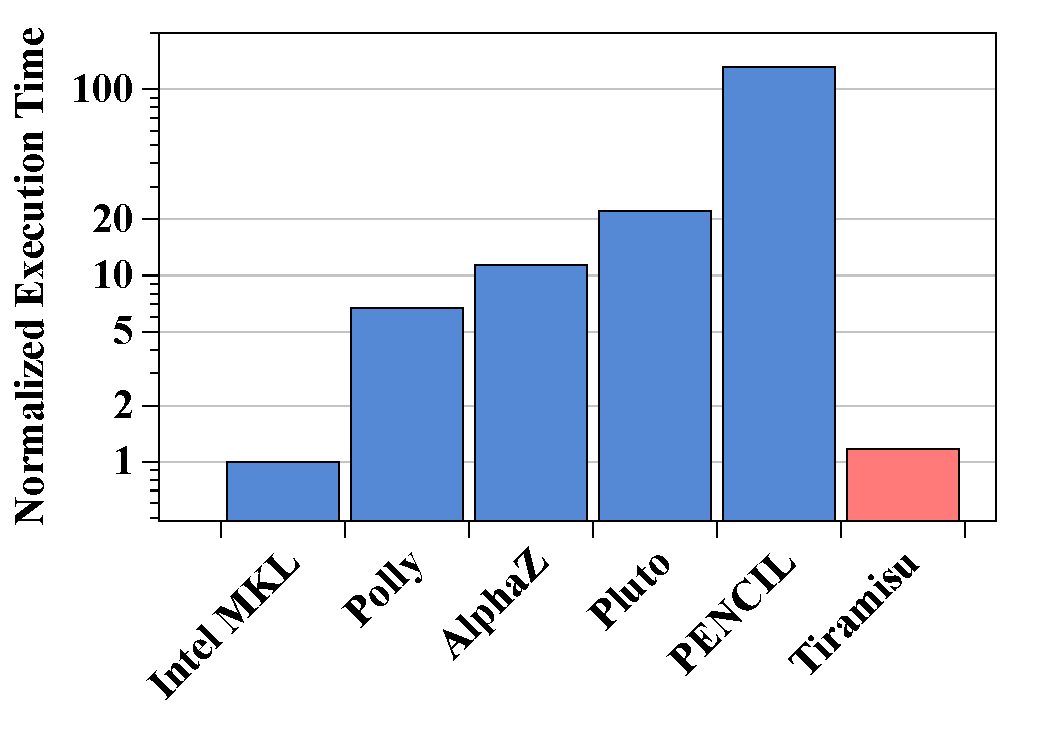
\includegraphics[width=\columnwidth]{./figures/sgemm_performance_CPU.pdf}
  \end{minipage}
  \begin{minipage}{0.22\textwidth}
    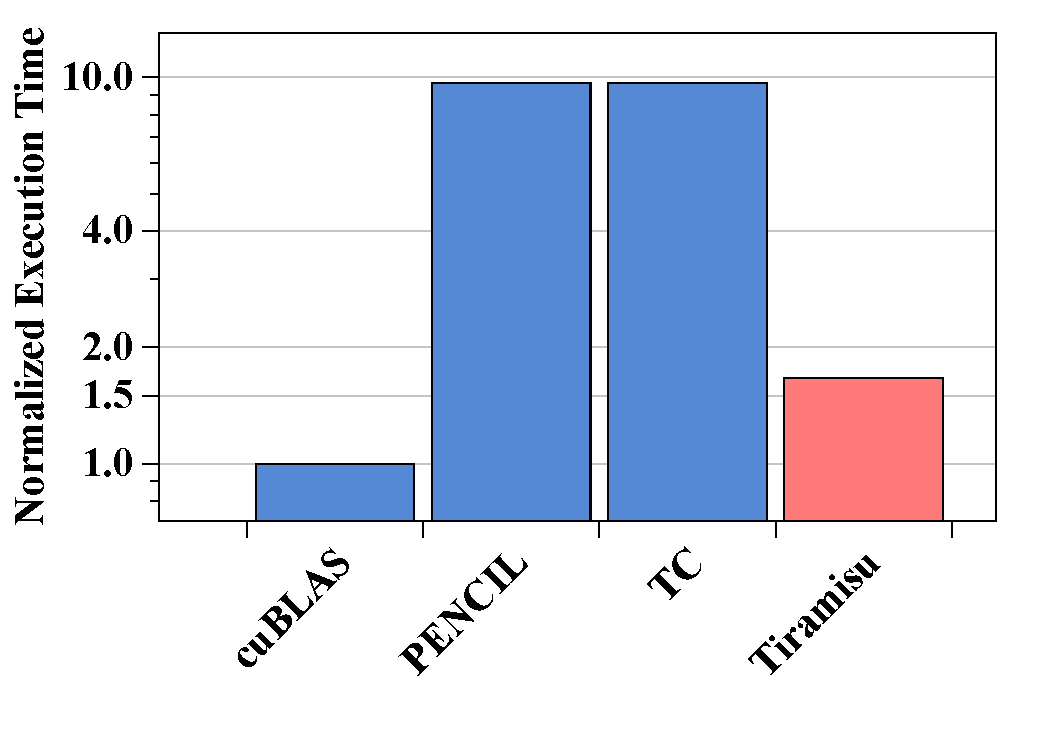
\includegraphics[width=\columnwidth]{./figures/sgemm_performance_GPU.pdf}
  \end{minipage}
  \vspace{-0.5cm}
  \caption{Normalized execution times of code generated for \texttt{sgemm} on CPU (left) and GPU (right).}
  \label{gemm-cpu-gpu}
  \vspace{-0.5cm}
\end{figure}

Previous work using the polyhedral model has shown success in implementing complex iteration space transformations~\cite{wolf1991loop,bondhugula_practical_2008,trifunovic_graphite_2010,polly,Vasilache2018TensorCF}, data locality optimizations~\cite{Iri88,tobias_hexagonal_cgo13}, and memory management optimizations~\cite{feautrier_array_1988,thies_unified_2001,lefebvre_automatic_1998,Qui00,Darte_contraction_2005}.
Although polyhedral compilers are able to represent these program and data transformations and generate complex code, they are still not successful in selecting transformations for the best performance. They still do not match the performance of highly hand-optimized kernels such as \texttt{gemm}. Blue bars in Figure~\ref{gemm-cpu-gpu} show the performance of state-of-the-art polyhedral compilers for \texttt{gemm} compared to the Intel MKL~\cite{mkl} and Nvidia cuBLAS~\cite{cublas} libraries.
Fully-automatic polyhedral compilers such as Polly~\cite{polly}, Pluto~\cite{bondhugula_practical_2008}, and PENCIL~\cite{pencil_paper,pencil_pact} improve productivity, but fail to obtain the desired level of performance since their search techniques consider only a subset of the necessary optimizations and they rely on less accurate machine models, leading the compiler to make suboptimal decisions.
Other polyhedral frameworks, such as AlphaZ~\cite{yuki2012alphaz} and CHiLL~\cite{chill}, eschew full automation and instead expose a \textit{scheduling language} that enables users to productively explore the space of possible transformations.
While these frameworks achieve better performance, their scheduling languages are not designed to target GPUs and distributed systems. For example, they do not allow the user to partition computations, send data across nodes, map buffers to GPU shared or local memory,  or insert required synchronization.

In this paper, we introduce \framework{}, the first polyhedral compiler with a scheduling language featuring \emph{novel extensions for targeting multiple high performance architectures}.
\framework{} is well suited for implementing data parallel algorithms (loop nests manipulating arrays).
It takes a high level representation of the program (pure algorithm and a set of scheduling commands), applies the necessary code transformations, and generates highly-optimized code for the target architecture.   
In addition to scheduling commands for loop and data-layout transformations, the \framework{} scheduling language introduces novel commands for computation partitioning, explicit communication and synchronization, and for mapping buffers to different memory hierarchies.
In order to simplify the implementation of the scheduling language, \framework{} explicitly divides the intermediate representation into four layers designed to hide the complexity and large variety of execution platforms by separating the architecture-independent algorithm from the code transformations, data-layout, and communication.

%\framework{} differs from prior similar compilers in many respects.  Unlike fully-automatic polyhedral compilers, \framework{} does not rely on machine models and heuristics since these are not always accurate, instead it exposes mechanisms for applying transformations allowing the user to fully control scheduling.  Thanks to this difference, \framework{} can generate more efficient code as shown with the red bars in Figure~\ref{gemm-cpu-gpu}.
The use of a scheduling language has been shown to be effective for generating efficient code by multiple compilers including CHiLL, AlphaZ, and Halide~\cite{halide_12,DBLP:conf/pldi/Ragan-KelleyBAPDA13}. Halide is the most successful example as it is now used in production by multiple companies.
%\framework{} expands existing scheduling languages with a set of novel scheduling commands that allow users to generate more efficient code for a richer set of execution environments, including GPUs, FPGAs, and distributed machines.  Its scheduling language features novel commands for controlling data communication, synchronization and for mapping to different memory hierarchies.
In comparison with Halide in particular, not only does \framework{} introduce novel scheduling extensions, it also fundamentally differs from Halide in that \framework{} relies on the expressive polyhedral representation instead of the interval-based representation used by Halide.  This allows \framework{} to express non-rectangular iteration spaces, to support programs with cyclic data-flow graphs, and to apply any affine transformation (including iteration space skewing), all of which are not possible in Halide.

This paper makes the following contributions:

\begin{itemize}
  \item We introduce a polyhedral compiler with a scheduling language that features \emph{novel extensions for controlling data communication, synchronization, and for mapping to different memory hierarchies}.  These extensions enable targeting multiple high-performance architectures including multicore CPUs, GPUs, and distributed machines.

   % We explicitly divide the IR into 4 layers to simplify the implementation ...
  \item We explicitly divide the intermediate representation into four layers to simplify the implementation of the scheduling language.  The four-layer IR separates the algorithm from code transformations and data-layout transformations, allowing for portability and simplifying the composition of architecture-specific lowering transformations.

  \item We evaluate \framework{} on a set of image processing and stencil benchmarks and compare it with Halide, an industrial compiler with a scheduling language, and with PENCIL, a state-of-the-art polyhedral compiler.  We show that Tiramisu matches or outperforms existing compilers on different hardware architectures, including multicore CPUs, GPUs, and distributed machines.
\end{itemize}

%TODO: unify scheduling language term.


\vspace*{-0.25cm}
\section{Related Work\label{related}}
\vspace*{-0.1cm}
\paragraph{Polyhedral compilers with automatic scheduling.}

Polyhedral compilers such as PENCIL~\cite{pencil,pencil_paper}, Pluto~\cite{bondhugula_practical_2008}, Polly~\cite{polly}, Tensor Comprehensions~\cite{Vasilache2018TensorCF}, and PolyMage~\cite{Mullapudi:2015:PAO:2786763.2694364} are fully automatic.  Some of them are designed for specific domains (such as Tensor Comprehensions and PolyMage), while Pluto, PENCIL, and Polly are more general.
While such fully automatic compilers provide productivity, they may not always obtain the best performance.  This is due to many reasons: first, these compilers do not implement some key optimizations such as array packing~\cite{Goto:2008:AHM:1356052.1356053}, register blocking, data prefetching, and asynchronous communication (which are all supported by \framework{}); second, they do not have a precise cost-model to decide which optimizations are profitable.  For example, the Pluto~\cite{bondhugula_practical_2008} automatic scheduling algorithm (which is used for automatic scheduling in Pluto, PENCIL, Polly, and Tensor Comprehensions) tries to minimize the distance between producer and consumer statements while maximizing outermost parallelism, but it does not consider the data layout, redundant computations, or the complexity of the control of the generated code.  PolyMage uses a custom scheduling algorithm designed for image processing code, but such an algorithm does not address all the complexities that arise when targeting GPUs and distributed systems.
Instead of fully automatic scheduling, \framework uses a more pragmatic approach and relies on a set of scheduling commands, giving the user full control over scheduling.

% and to map buffers to the right memory hierarchy level; it needs to decide about the correctness of non-affine and data-layout transformations; it needs ; and it needs a sophisticated search technique to search efficiently the very large space of optimizations.  

Polyhedral frameworks proposed by ~\citet{Amarasinghe:1993:COC:173262.155102} and~\citet{6877466} address the problem of code generation for distributed systems. \framework{} makes a different design choice, relying on the user to provide scheduling commands to control choices in the generated code (synchronous/asynchronous communication, the granularity of communication, buffer sizes, when to send and receive, the cost of communication versus re-computation, etc.).

Even though \framework{} focuses on providing mechanisms for code optimization, it is still possible to build a framework that provides policy on top of \framework{} (i.e., a framework that automates scheduling).  This separation provides flexibility, making it possible to plug in different policies depending on user requirements.  %The separation between mechanism and policy allows users to choose between using automatic scheduling or manual scheduling which provides more flexibility.

%\vspace*{-0.3cm}
\paragraph{Polyhedral compilers with a scheduling language.}
AlphaZ~\cite{yuki2012alphaz}, CHiLL~\cite{chill,Hall2010}, URUK~\cite{Girbal2006}, and Transformation Recipes~\cite{Hall:2009:LTR:2155247.2155251} are polyhedral frameworks and methods developed to allow users to express high-level transformations using scheduling commands. 
Since these frameworks are polyhedral, they can express any affine transformation.
Their scheduling languages do not target distributed architectures, however, nor do they target GPUs (except the Transformation Recipes framework).  In comparison with these frameworks, \framework features scheduling commands for partitioning computations for execution on a distributed system, synchronization, distribution of data across nodes, mapping data to specific GPU memory hierarchy levels, and performing array packing.  The first four columns of Table~\ref{tab:related} show a summary of a comparison between \framework{} and three representative polyhedral frameworks.

\begin{table}[tb]
    \scriptsize
    \setlength\tabcolsep{1pt}
    \begin{tabular}{l|l|l|l|l|l}
        \hline
        
        \textbf{Feature} & \textbf{Tiramisu} & \textbf{AlphaZ} & \textbf{PENCIL} & \textbf{Pluto} & \textbf{Halide} \\\hline

        \textbf{CPU code generation} & \yes & \yes & \yes & \yes  & \yes \\\hline

        \textbf{GPU code generation} & \yes & \no & \yes & \yes  & \yes \\\hline

        \textbf{Distributed CPU code generation} & \yes & \no & \no & \yes  & \yes\\\hline
        
        \textbf{Distributed GPU code generation} & \yes & \no & \no & \no  & \no\\\hline

        \textbf{Support all affine loop transformations} & \yes & \yes & \yes & \yes  & \no\\\hline

        \textbf{Optimize data accesses} & \yes & \yes & \no & \no & \yes \\\hline

        \textbf{Commands for loop transformations} & \yes & \yes & \no & \no & \yes\\\hline

        \textbf{Commands for optimizing data accesses} & \yes & \yes & \no & \no & \yes \\\hline

        \textbf{Commands for performing data copies} & \yes & \no & \no & \no & \no \\\hline

        \textbf{Commands for memory hierarchies} & \yes & \no & \no & \no & \limited\\\hline

        \textbf{Expressing cyclic data-flow graphs} & \yes & \yes & \yes & \yes & \no \\\hline

        \textbf{Support non-rectangular iteration spaces} & \yes & \yes & \yes & \yes & \limited\\\hline

        \textbf{Instance-wise, exact dependence analysis} & \yes & \yes & \yes & \yes  & \no\\\hline
        
        \textbf{Compile-time affine-set emptiness check} & \yes & \yes & \yes & \yes  & \no\\\hline

        \textbf{Implement support for parametric tiling} & \no & \yes & \no & \no  & \yes\\\hline
    \end{tabular}
    \caption{Comparison Between Different Frameworks.}
    \label{tab:related}
    \vspace{-0.75cm}
\end{table}

\paragraph{Non-polyhedral compilers with a scheduling language.}
Halide~\cite{halide_12} is an image processing DSL that has a scheduling language; however, it uses intervals to represent iteration spaces instead of the polyhedral model.  This limits the expressiveness of Halide.
For example, Halide cannot naturally represent non-rectangular iteration spaces.  This makes certain Halide passes over-approximate non-rectangular iteration spaces, potentially leading to less efficient code.  It also makes Halide over-approximate the amount of data to communicate (send and receive) when generating distributed code,  and also prevents Halide from performing precise bounds inference for non-rectangular iteration spaces, as well as performing many complex affine transformations, such as iteration space skewing, which are all possible in \framework{}.

Halide does not have dependence analysis and thus it relies on conservative rules to determine whether a schedule is legal; for example, Halide does not allow the fusion of two loops (using the \texttt{compute\_with} command) if the second loop reads a value produced by the first loop.
While this rule avoids illegal fusion, it prevents fusing many legal common cases which may lead to suboptimal performance.
Halide also assumes the program has an acyclic dataflow graph in order to simplify checking the legality of a schedule. This prevents users from expressing many programs with cyclic dataflow.
It is possible in some cases to work around the above restrictions, but such methods are not general.
\framework{} avoids over-conservative constraints by relying on dependence analysis to check for the correctness of code transformations, enabling more possible schedules.  Table~\ref{tab:related} shows a comparison between \framework{} and Halide.

Other systems include POET~\cite{Yi:2007ay}, which uses an XML-based description of code and transformation behavior to parametrize loop transformations.  It uses a purely-syntactic transformation system to produce transformed code.  The use of syntactic transformations is less general than the polyhedral model used in \framework.

\paragraph{Non-polyhedral compilers with automatic scheduling.}

Delite \cite{chafi_domain-specific_2011} is a generic
framework for building DSL compilers using Lightweight Modular Staging (LMS) \cite{lms_staging_10}. It exposes several parallel computation patterns that DSLs can use to express parallelism.
NOVA~\cite{Collins:2014:NFL:2627373.2627375} and Lift~\cite{Steuwer:2017:LFD:3049832.3049841} are other IRs for DSL compilers.  They are functional languages that rely on a suite of higher-order functions such as map, reduce, and scan to express parallelism.
Weld~\cite{palkar2017weld} is another IR designed for the area of databases and data analytics and can be used to implement libraries, such as Numpy~\cite{numpy}, and enable optimizations across different library calls.
\framework{} is complementary to all of these frameworks as \framework{} would allow them to perform and compose a large set of complex affine transformations that are easier to express in the polyhedral model.

%The Cyclops Tensor Framework (CTF)~\cite{solomonik2013cyclops} is a library for performing tensor contractions, primarily in the field of quantum chemistry. CTF automatically decomposes tensors using a communication-optimal tensor contraction algorithm and maps the computations to the underlying architecture. The framework targets distributed architectures, and can provide hybrid execution through the use of MPI and OpenMP.  Unlike \framework{} which is designed to be more general, CTF is designed mainly for tensor contractions.
%Chapel~\cite{Chamberlain:2007:PPC:1286120.1286123} is a parallel programming language that supports a Partitioned Global Address Space (PGAS) memory model~\cite{Krishnamurthy:1993:PPS:169627.169724}.  In this model, code can refer to variables and arrays regardless of whether they are stored in a local or remote memory.  Any necessary communication is automatically inserted by the compiler and executed at runtime.  Similarly, computations in Layer I of \framework{} refer to other computations in the same way regardless of whether they are stored or computed in local or remote memory (or in shared or global memory on GPU).  Specifying whether a computation is local or remote, how it is accessed and whether communication is needed are all done using scheduling commands at Layers II, III and IV. \framework{} provides a set of fine-grain commands that can implement any data-mapping and communication that a language like Chapel provides, yet \framework{} can complement Chapel by providing new capabilities such as advanced loop nest transformations and checking schedule validity.
% large has the advantage of enabling manual scheduling, data mapping and communication (while Chapel.


\vspace{-0.25cm}
\section{The \framework Embedded DSL}

\framework{} is a domain-specific language (DSL) embedded in C++. It provides a pure C++ API that allows users to write a high level, architecture-independent algorithm and a set of scheduling and data mapping commands that guide code generation.
The input \framework code can either be written directly by a programmer, or generated by a different DSL compiler.  \framework{} then constructs a high level intermediate representation (IR), applies the user-specified code and data-layout transformations, and generates optimized backend code (LLVM IR and CUDA) that takes advantage of the target hardware features.


\vspace{-0.25cm}
\paragraph{\textbf{Scope}}
\framework is designed for expressing data parallel algorithms, especially those that operate over dense arrays using loop nests and sequences of statements.  These algorithms are often found in the areas of dense linear algebra and tensor algebra, stencil computations, image processing, and deep neural networks.

\vspace{-0.3cm}
\subsection{Specifying the Algorithm}
The first part of a \framework{} program specifies the algorithm without specifying the schedule (when and where the computations occur), how data should be stored in memory (data-layout), or communication.
At this level there is no notion of data location; rather, values are communicated via explicit producer-consumer relationships.

The algorithm is a pure function that has inputs, outputs, and a sequence of statements.  The statements are called \textit{computations} in \framework.  Flow-control around these computations is restricted to \texttt{for} loops and conditionals;  \texttt{while} loops, early exits and \texttt{GOTO}s cannot be expressed.  To declare a computation, the user provides both the iteration domain of the computation and the expression to compute.  %In the rest of this section, we will provide an example of the API used to declare computations in \framework.

Figure~\ref{fig:algorithm} shows a blur algorithm written in \framework, using \texttt{bx} and \texttt{by}, which are the two computations in this algorithm.
The first computation, \texttt{bx}, computes a horizontal blur of the input, while the second computation, \texttt{by}, computes the final blur \texttt{by} averaging the output of the first stage.
The iterators \texttt{i}, \texttt{j} and \texttt{c} in line~\ref{fig:example:tiramisu:iterators} define the iteration domain of \texttt{bx} and \texttt{by} (for brevity we ignore boundary conditions).
The algorithm is semantically equivalent to the following code.
%By default, all of the computed values are stored in memory. Each computation has an implicit buffer associated with it where the number of dimensions of this buffer is equal to the number of dimensions in the iteration domain.

\begin{figure}
\begin{lstlisting}[language=C,escapechar=@]
// Declare the iterators i, j and c.
var i(0, N-2), j(0, M-2), c(0, 3);@\label{fig:example:tiramisu:iterators}@

// Algorithm.
bx(i,j,c) = (in(i,j,c)+in(i,j+1,c)+in(i,j+2,c))/3;@\label{fig:example:tiramisu:computation1}@
by(i,j,c) = (bx(i,j,c)+bx(i+1,j,c)+bx(i+2,j,c))/3@\label{fig:example:tiramisu:computation2}@);
\end{lstlisting}
\vspace{-0.25cm}
\caption{\label{fig:algorithm}\texttt{Blur} algorithm without scheduling commands.}
\vspace{-0.25cm}
\end{figure}

\begin{lstlisting}[language=C,escapechar=@]
for (i in 0..N-2)
 for (j in 0..M-2)
  for (c in 0..3)
   bx[i][j][c] = (in[i][j][c]+in[i][j+1][c]+in[i][j+2][c])/3
for (i in 0..N-2)
 for (j in 0..M-2)
  for (c in 0..3)
   by[i][j][c] = (bx[i][j][c]+bx[i+1][j][c]+bx[i+2][j][c])/3
\end{lstlisting}


\vspace{-0.25cm}
\subsection{Scheduling Commands}

\framework provides a set of high-level scheduling commands for common optimizations. Table~\ref{tab:scheduling} shows examples of these commands.  There are four types of scheduling commands:
\begin{itemize}
    \item Commands for loop nest transformations: they include common affine transformations such as loop tiling, splitting, shifting, etc.  For example, applying a 32$\times$32 loop tiling on a computation \texttt{C} can be done by calling\\ \texttt{C.tile(i,j,32,32,i0,j0,i1,j1)} where \texttt{i} and \texttt{j} are the original loop iterators and \texttt{i0}, \texttt{j0}, \texttt{i1}, and \texttt{j1} are the names of the loop iterators after tiling.

    \item Commands for mapping loop levels to hardware: these include loop parallelization, vectorization, mapping loop levels to a GPU block or thread dimension. For example calling \texttt{C.vectorize(j, 4)} splits the \texttt{j} loop by a factor of 4 and then maps the inner loop to vector  instructions.

    \item Commands for manipulating data: these include (1) allocating arrays; (2) setting array properties including whether the array is stored in host, device, shared, or local memory (GPU); (3) copying data (between levels of memory hierarchies or between two nodes);  (4) setting array accesses. In most cases, users need only use high level commands for data manipulation. If the high level commands are not expressive enough, the user can use the more expressive low level commands.

    \item Commands for adding synchronization operations: the user can either declare a barrier or use the \texttt{send} and \texttt{receive} functions for point-to-point synchronization.
\end{itemize}

\begin{table}[t]
    \scriptsize
    \setlength\tabcolsep{1pt}
    \begin{tabular}{l|l}
        \hline
        \multicolumn{2}{c}{\textbf{We assume that C and P are computations, b is a buffer, i and j are loop iterators}} \\\hline
        \multicolumn{2}{c}{\textbf{Commands for loop nest transformations}} \\\hline
        \textbf{Command} & \textbf{Description} \\\hline
        \begin{tabular}{ll} \texttt{C.tile(}& \texttt{i,j,t1,t2,}\\ & \texttt{i0,j0,i1,j1)}
        \end{tabular} & 
        \begin{tabular}{l}
        Tile the dimensions (i,j) of the computation C by $t1\times t2$.\\
        The names of the new dimensions are (i0, j0, i1, j1), where \\
        (i0, j0) are the outer tiles and (i1, j1) are the inner tiles.\end{tabular}\\ \hline
        \texttt{C.interchange(i, j)} & Interchange the dimensions of C (loop interchange) \\\hline
        \texttt{C.shift(i, s)} & Loop shifting (shift the dimension i by s iterations) \\ \hline
        \texttt{C.split(i, s, i0, i1)} & Split the dimension i by s. (i0, i1) are the new dimensions\\ \hline
        \texttt{P.compute}\_at(C, j) & Compute the computation \emph{P} in the loop nest of \emph{C} at loop\\
        & level j.  This might introduce redundant computations.\\
        \hline
        \texttt{C.unroll(i, v)} & Unroll the dimension i by a factor v\\\hline
        \texttt{C.after(B, i)} & Indicate that C should be ordered after B at the loop level i\\
        &(they have the same order in all the loop levels above i)\\
        \hline
        \texttt{C.inline()} & Inline C in all of its consumers\\ \hline
        \texttt{C.set\_schedule()} & Set an affine transformation for C (to transform Layer I to II)\\\hline
        \multicolumn{2}{c}{\textbf{Commands for mapping loop levels to hardware}} \\\hline
        \texttt{C.parallelize(i)} & Mark the dimension i as a space dimension (cpu)\\\hline
        \texttt{C.vectorize(i, v)} & Vectorize the dimension i by a vector size v\\\hline
        \texttt{C.gpu(i0, i1, i2)} & Mark the dimensions i0, i1 and i2 to be executed on the GPU \\\hline
        \texttt{C.tile\_gpu(i0, i1)} & Tile the loops i0 and i1 and map them to GPU \\\hline
        \texttt{C.distribute(i)} & Mark the dimension i as a space dimension (node)\\\hline
        \multicolumn{2}{c}{\textbf{High level commands for data manipulation}} \\\hline
        \texttt{\textbf{C.store\_in(b,\{i, j\})}} & Store the result of the computation C(i,j) in b[i,j].\\\hline
        \texttt{\textbf{C.cache\_shared\_at(C, i)}} & Cache (copy) the buffer of C in shared memory. The amount\\
        & of data to copy, the access functions, and synchronization are\\
        & computed automatically.\\\hline
        \texttt{\textbf{C.cache\_local\_at(C, i)}} & Similar to \texttt{cache\_shared\_at} but stores in local GPU memory.\\\hline
        \texttt{\textbf{send(d, src, s, q, p)}}
            & Create a send operation. \texttt{d}: vector of iterators to represent \\
            &  the iteration domain; \texttt{src}: source buffer; \texttt{s}: size; \texttt{q}: destination \\
            & node; \texttt{p}: properties (synchronous/asynchronous, blocking, ...).
        \\\hline
        \texttt{\textbf{receive(d, dst, s, q, p)}}
            & Create a receive operation. Arguments similar to \texttt{send} except\\
            &\texttt{q} which is the source node.
        \\\hline
        \multicolumn{2}{c}{\textbf{Low level commands for data manipulation}}\\\hline
        \texttt{\textbf{Buffer b(sizes, type)}} & Declare a buffer (\texttt{s}: a vector of dimension sizes, \texttt{t}: type). \\\hline
        \texttt{\textbf{b.allocate\_at(p, i)}} & Return an operation that allocate b at the loop i of p.\\\hline
        \texttt{\textbf{C.buffer()}} & Return the buffer associated to the computation C.\\\hline
        \texttt{\textbf{b.set\_size(sizes)}} & Set the size of a buffer. \texttt{sizes}: a vector of dimension sizes.\\\hline
        \texttt{\textbf{b.tag\_gpu\_global()}} & Tag this buffer to be stored in global GPU memory.\\\hline
        \texttt{\textbf{b.tag\_gpu\_shared()}} & Tag this buffer to be stored in shared GPU memory.\\\hline
        \texttt{\textbf{b.tag\_gpu\_local()}} & Tag this buffer to be stored in local GPU memory.\\\hline
        \texttt{\textbf{b.tag\_gpu\_constant()}} & Tag this buffer to be stored in constant GPU memory.\\\hline
        \texttt{\textbf{C.host\_to\_device()}} & Return an operation that copies C.buffer() from host to device.\\\hline
        \texttt{\textbf{C.device\_to\_host()}} & Return an operation that copies C.buffer() from device to host.\\\hline
        \texttt{\textbf{copy\_at(p, i, bs, bd)}}
            & Return an operation that copies the buffer \texttt{bs} to the buffer \texttt{bd} at\\
            & the loop i of p.
            Used for copies between global, shared and local.
        \\\hline
        \multicolumn{2}{c}{\textbf{Commands for synchronization}} \\\hline
        \texttt{\textbf{barrier\_at(p, i)}}
            & Create a barrier at the loop p of i.
        \\\hline
    \end{tabular}
    \caption{Examples of \framework{} Scheduling Commands}
    \label{tab:scheduling}
    \vspace{-0.75cm}
\end{table}

The novel commands that \framework introduces are highlighted in \textbf{bold} in Table~\ref{tab:scheduling}.  They include array allocation, copying data between memory hierarchies, sending and receiving data between nodes, and synchronization.  Calls to \texttt{cache\_shared\_at()}, \texttt{cache\_local\_at()}, \texttt{allocate\_at()}, \texttt{copy\_at()}, \texttt{barrier\_at()} return an operation that can be scheduled like any other computation.
The operations \\ \texttt{cache\_shared\_at()} and \texttt{cache\_local\_at()} can be used to create a cache for a buffer (GPU only).  They automatically compute the amount of data that needs to be cached, perform the data copy, and insert any necessary synchronization.

\begin{figure*}[t]
    \centering
    \scriptsize
    \setlength\tabcolsep{4pt}
\begin{tabular}{cl|@{}l}
 &
    \ \ \ \ \ \ \ \ \ \ \ \ \ \ \ \ \ \ \ \ \ \ \ \ \ \ \ \ \ \ \ \ \ \ \ 
    \textbf{\framework Scheduling Commands}
 &
    \ \ \ \ \ \ \ \ \ \ \ \ \ \ \ \ \ \ \ \ \ \
    \textbf{Pseudocode Representing Code Generated by \framework}
\\\hline

{\textbf{\normalsize(a)}} &

\begin{lstlisting}[language=C,escapechar=@]
// Scheduling commands for targeting GPU.
// Tile i and j and map the resulting dimensions to GPU
var i0, j0, i1, j1;
by.tile_gpu(i, j, 32, 32, i0, j0, i1, j1);
bx.compute_at(by, j0);
bx.cache_shared_at(by, j0);

// Use struct-of-array data layout for bx and by.
bx.store_in({c,i,j}); by.store_in({c,i,j});

// Create data copy operations
operation cp1 = in.host_to_device();
operation cp2 = by.device_to_host();

// Specify the order of execution of copies
cp1.before(bx, root); cp2.after(by, root);
\end{lstlisting}

%%%%%%%%%%%%%%%%%%%%%%%%%%%%%%%%%%%%%%%%%%%%%%%

& 

\begin{lstlisting}[language=C,escapechar=@]
 host_to_device_copy(in_host, in);

 @{\color{listingkeywordcolor}{\textbf{GPUBlock}}}@ for(i0 in 0..floor(N-2,32))
  @{\color{listingkeywordcolor}{\textbf{GPUBlock}}}@ for(j0 in 0..floor(M-2,32))
   @{\color{listingkeywordcolor}{\textbf{shared}}}@ bx[3,32,34];
   @{\color{listingkeywordcolor}{\textbf{GPUThread}}}@ for(i1 in 0..min(N-2,32*i0+31+2))
    @{\color{listingkeywordcolor}{\textbf{GPUThread}}}@ for(j1 in 0..min(M-2,32*j0+31+2))
     for (c in 0..3)
      bx[c][i1-32*i0][j1-32*j0]=
        (in[i1][j1][c]+in[i1][j1+1][c]+in[i1][j1+2][c])/3@\label{fig:motivating:code2:stmt2}@
   @{\color{listingkeywordcolor}{\textbf{GPUThread}}}@ for(i1 in 0..min(N-2,32*i0+31))
    @{\color{listingkeywordcolor}{\textbf{GPUThread}}}@ for(j1 in 0..min(M-2,32*j0+31))
     for (c in 0..3)
      by[c][i1][j1]=(bx[c][i1][j1]+bx[c][i1+1][j1]+bx[c][i1+2][j1])/3@\label{fig:motivating:code2:stmt3}@

 device_to_host_copy(by, by_host);

\end{lstlisting}
    
%%%%%%%%%%%%%%%%%%%%%%%%%%%%%%%%%%%%%%%%%%%%%%%

\\\hline
{\textbf{\normalsize(b)}} &
\begin{lstlisting}[language=C,escapechar=@]
// Scheduling commands for targeting a distributed system
// Declare additional iterators
var ii(0,2), jj(0,M), qs(1,RANKS), qr(0,RANKS-1), q, z;

// Split loop i into loops q and z and parallelize z
bx.split(i,N/RANKS,q,z); bx.parallelize(z);@\label{line:split1}@
by.split(i,N/RANKS,q,z); by.parallelize(z);@\label{line:split2}@ 

// Create communication and order execution
send s = send({qs}, bx(0,0,0), 2xMx3, qs-1, {ASYNC});@\label{line:send}@
recv r = receive({qr}, bx(N,0,0), 2xMx3, qr+1, 
                 {SYNC}, s);@\label{line:recv}@
s.before(r,root); r.before(bx,root)

// Distribute the outermost loops
bx.distribute(q); by.distribute(q); @\label{line:comp_dist}@
s.distribute(qs); r.distribute(qr); @\label{line:comm_dist}@
\end{lstlisting}
%%%%%%%%%%%%%%%%%%%%%%%%%%%%%%%%%%%%%%%%%%%%%%%
% // qs-1 is the rank of the receiving node
%// qr+1 is the rank of the sending node

& 

%%%%%%%%%%%%%%%%%%%%%%%%%%%%%%%%%%%%%%%%%%%%%%%

\begin{lstlisting}[language=C,escapechar=@]

 @{\color{listingkeywordcolor}{\textbf{distributed}}}@ for (qs in 1..RANKS) @\label{line:distfor}@
   send(bx(0,0,0), 2xMx3, qs-1,{ASYNC,BLK})
 @{\color{listingkeywordcolor}{\textbf{distributed}}}@ for (qr in 0..RANKS-1)
   recv(bx(N,0,0), 2xMx3, qr+1, {SYNC,BLK})

 @{\color{listingkeywordcolor}{\textbf{distributed}}}@ for (q in 0..RANKS)
   @{\color{listingkeywordcolor}{\textbf{parallel}}}@ for (i in 0..N/RANKS)
    for (j in 0..M)
      for (c in 0..3)
        bx[i][j][c] = (in[i][j][c]+in[i][j+1][c]+in[i][j+2][c])/3@\label{fig:motivating:code2:stmt1}@
 @{\color{listingkeywordcolor}{\textbf{distributed}}}@ for (q in 0..RANKS)
   @{\color{listingkeywordcolor}{\textbf{parallel}}}@ for (i in 0..N/RANKS)
    for (j in 0..M)
      for (c in 0..3)
        by[i][j][c] = (bx[i][j][c]+bx[i+1][j][c]+bx[i+2][j][c])/3
\end{lstlisting}

%%%%%%%%%%%%%%%%%%%%%%%%%%%%%%%%%%%%%%%%%%%%%%%

\\\hline
\end{tabular}
\vspace{-0.25cm}
\caption{Two examples illustrating \framework{} scheduling commands (left) and the corresponding generated code (right). (a) presents a set of scheduling commands for mapping to GPU; (b) presents a set of scheduling commands for mapping to a distributed CPU machine}
\label{fig:mainexample}
\vspace{-0.25cm}
\end{figure*}


The use of \texttt{allocate\_at()}, \texttt{copy\_at()}, and \texttt{barrier\_at()} allows \framework to automatically compute iteration domains for the data copy, allocation, and synchronization operations.  This is important because it relieves the user from guessing and computing the iteration domain manually, especially when exploring different possible schedules.  To illustrate this, consider the example of copying a buffer from global memory to shared memory in a loop nest executing on a GPU.  The size of the area to copy and the iteration domain of the copy operation itself (which is a simple assignment in this case) depends on whether the loop is tiled, the tile size, and  whether any other loop transformation has already been applied. Computing the size of the area to copy in this case is not trivial.  \framework simplifies this step by computing the iteration domain and the area of data to be copied from the schedule directly.

To illustrate more \framework{} scheduling commands, let us take the \texttt{blur} example again from Figure~\ref{fig:algorithm},
and map the two outermost loops of \texttt{bx} and \texttt{by} to GPU.  The necessary scheduling commands are shown in Figure~\ref{fig:mainexample}-\codetwo{} (left).
The \texttt{tile\_gpu()} command tiles the computations then maps the new loops to GPU block and thread dimensions.  The \texttt{compute\_at()} command computes the tiles of \texttt{bx} that need to be read by \texttt{by}.  This transformation introduces redundant computations (in this case) and is known as overlapped tiling~\cite{Krishnamoorthy:2007:EAP:1273442.1250761}.
\texttt{cache\_shared\_at()} instructs \framework to store the results of the \texttt{bx} computation in shared memory.
The subsequent scheduling command (\texttt{store\_in()}) specifies the access functions of \texttt{bx} and \texttt{by}.  In this case, it indicates that these computations are stored in a SOA (struct-of-array) data layout (to allow for coalesced accesses).  The final commands create data copy operations (host-to-device and device-to-host) and schedule them.

Suppose we want to distribute the \texttt{blur} example and run it on a distributed system with multicore CPU nodes. Figure \ref{fig:mainexample}-\codethree{} (left) shows the scheduling commands to use in this case. The \texttt{split()} command splits the outer loop, \texttt{i}, of \texttt{bx} by a splitting factor of \texttt{N/RANKS}.  It creates two new loops \texttt{q} and \texttt{z} such that the outer loop, \texttt{q}, iterates over the number of \texttt{RANKS} (i.e. the number of processes we want to distribute).  The \texttt{q} loop iterator will be mapped later to an MPI \texttt{rank}.  We also parallelize the new inner loop, \texttt{z}, and perform the same transformations on \texttt{by}.

\texttt{create\_send()} and \texttt{create\_recv()} define communication, which in this case, sends $2\times M \times3$ contiguous data elements between nodes starting from \texttt{bx(0,0,0)}. The receiving node consumes the sent data starting from \texttt{bx(N,0,0)}. \texttt{qs} and \texttt{qr} represent the iteration domains. \texttt{qs-1} and \texttt{qr+1} represent the send's destination node and the receive's source node, respectively. \texttt{\{ASYNC\}} defines an asynchronous send and \texttt{\{SYNC\}} defines a synchronous receive.
In this example, we explicitly specify the send and receive operations for illustrative reasons, instead of relying on \framework to automatically insert them.
Explicit send and receive operations are only useful if the array accesses or the iteration domain are not affine (more details about non-affine code in Sec.\ref{nonaffine}) because in such cases automatically computing the amount of data to exchange may not be accurate (the experimental section shows such cases).
Finally, we tag the appropriate loops (the outer loops of \texttt{bx}, \texttt{by}, \texttt{s}, and \texttt{r}), to be distributed (i.e., we tag each iteration to be run on a different node).

%Internally, these distributed \texttt{for} loops (shown in \ref{fig:mainexample}-\codethree{} on the right) will become \texttt{if} statements that check the rank of the currently executing process to see if it is within the range of allowed ranks. For example, the \texttt{distributed for} loop on line \ref{line:distfor} would internally become \texttt{qs=get\_rank();} \texttt{if} \texttt{(qs>=1} \texttt{and} \texttt{qs<RANKS)} \texttt{then... }
% A pseudocode of the code that we which to generate is shown in the right side of the same figure.
% For this example, we want to distribute the computation such that each MPI \emph{rank} (process) operates on contiguous rows of input data. Each rank gets \lstinline{chunk_sz} rows. On line \ref{line:split}, the outer loop is split by \lstinline{chunk_sz}. The resulting inner loop ranges over the rows in the chunk, and the outer loop ranges over the number of MPI ranks we want to use.

% Line \ref{line:send} and \ref{line:recv} deal with communication. We assume that our image data is already distributed, thus only boundary rows need to be communicated among adjacent ranks. We use two-sided communication in \framework{}, meaning communication is done with pairs of \emph{send} and \emph{receive} statements. Line \ref{line:send} defines an asynchronous blocking send operation to processor q-1.  \lstinline{create_send} takes as input the send iteration domain (which also defines the size of data to send), destination rank, communication type, and access into the producer.  Line \ref{line:recv} defines the receive operation.

% Line \ref{line:comp_dist} tags dimension \lstinline{y1} of \lstinline{bx} and \lstinline{by} as distributed, and line \ref{line:comm_dist} tags dimension \lstinline{q} of the \lstinline{send} and \lstinline{receive} as distributed.

All the other scheduling commands in \framework{} can be composed with transfers and distributed loops, as long as the composition is semantically correct. 
%This means we can do everything from basic transformations such as tiling a transfer to more advanced transformations including specializing a distributed computation based on rank.

\input{tex/background}

\section{\label{sec:ir}The \framework{} IR}

%\subsection{Example}

%% Challenge of scheduling
%Figures~\ref{fig:example-ir}-\codetwo{} (Schedule) and ~\ref{fig:example-ir}-\codethree{} (Schedule) show how a simple collection of scheduling commands can map the architecture independent program into different architectural configurations. 

%% The MPI+OpenMP+CUDA Challenge
%Figure~\ref{fig:example-ir}-\codethree{} (left) shows an example where the algorithm is mapped to a GPU cluster using simple scheduling commands and without the need to change the algorithm or to write code in different languages and libraries.


\begin{figure*}[t!]
    \centering
    \scriptsize
    \setlength\tabcolsep{4pt}
\begin{tabular}{cl|@{}l}
\multicolumn{3}{c}{\textbf{Constraints:} \boldsymbol{$\ \ \ C_n: 0\leq i < N, \ \ \ \ \ \ C_m: 0\leq j < M, \ \ \ \ C_{m'}: 1\leq j < M-1, \ \ \ \ C_{k}: 0\leq c < 3, \ \ \ \ C_{q}: 0\leq q < NUM\_NODES$}}
\\\hline
  &
    \ \ \ \ \ \ \ \ \ \ \ \ \ \ \ \ \ \ \ \ \ \ \ 
    \textbf{Different Code Optimizations}
  &
    \ \ \ \ \ \ \ \ \ \ \ \ \ \  
    \textbf{\framework representation (Layer I, Layer II and Layer III)}
\\\hline

{\textbf{\normalsize(a)}} &
\begin{lstlisting}[language=C,escapechar=@]
// Original unoptimized code
for (i in 0..N)
  for (j in 0..M)
    for (c in 0..3)
      b1[j][c] = 1.5*img[i][j][c] // brightening @\label{fig:motivating:code1:stmt1}@
  for (j in 0..M )
    for (c in 0..2)
      b2[j][c] = clamp(b1[j][c], 0, 255)@\label{fig:motivating:code1:stmt2}@
  for (j in 1..M-1)
    for (c in 0..3)
      out[i][j][c] = (b2[j-1][c] + b2[j][c] + @\label{fig:motivating:code1:stmt3}@
                      b2[j+1][c])/3
\end{lstlisting}
    &  
\begin{tabular}{c|l}
\multirow{12}{1cm}{\textbf{Layer I}}
    & \\
    & \\
    & \\
    & \\
    & The constraints $C_n$, $C_m$ and $C_k$ are defined above.\\
    & {\color{listingmauve}{$\{b_1\ (i, j, c): C_n \wedge C_m \wedge C_k\} $}} \ \ \ :\ \ \ $1.5*img(i, j, c)$\\
    & {\color{listingmauve}{$\{b_2\ (i, j, c): C_n \wedge C_m  \wedge C_k\}$}} \ \ \ :\ \ \ $\ clamp(b_1(i, j, c), 0, 255)$ \\
    & {\color{listingmauve}{$\{out(i, j, c): C_n \wedge C_{m'} \wedge C_k\}$}} \ :\  \ \ $(b_2(i,j-1,c)+b_2(i,j,c)+b_2(i,j+1,c))/3$\\
    & \\
    & \\
    & \\
    & \\
\end{tabular}
    \\\hline
{\textbf{\normalsize(b)}} &
\begin{lstlisting}[language=C,escapechar=@]
// Code optimized for CPU
@{\color{listingkeywordcolor}{\textbf{parallel}}}@ for (i in 0..N)
  for (j in 0..M)
    for (c in 0..3)
      float t = 1.5*img[i][j][c]@\label{fig:motivating:code2:stmt1}@
      b2[i][j][c] = clamp(t, 0, 255)@\label{fig:motivating:code2:stmt2}@
  for (j in 1..M-1)
    for (c in 0..3)
      out[i][j][c] = (b2[i][j-1][c] + 
                      b2[i][j][c] +@\label{fig:motivating:code2:stmt3}@
                      b2[i][j+1][c])/3
\end{lstlisting}
    & 
\begin{tabular}{c|l}
 \multirow{3}{*}{\textbf{Schedule}}
 & $b_2$.after($b_1$, c)\\
 & $b_1$.parallel(i); \ \ $b_2$.parallel(i); \ \  $out$.parallel(i)\\
 & $b_1$.store\_in($t$); \ \ $b_2$.store\_in($buf_{b2}[i, j , c]$); \ \  $out$.store\_in($buf_{out}[i, j , c]$);\\
 \hline
 \multirow{6}{*}{\textbf{Layer II}}
    & {\color{listinggreen}{// Layer II generated from Layer I using the schedule}}\\
    & \\
    & {\color{listingmauve}{$\{\ b_1(i (cpu), 0, j, c, 0) : C_n \wedge C_m \wedge C_k\}$}}: $1.5*img(i, j, c)$\\
    & {\color{listingmauve}{$\{\ b_2(i (cpu), 0, j, c, 1): C_n \wedge C_m \wedge C_k\}$}} : $clamp(b_1(i, 0, j, c, 0), 0, 255)$\\
    & {\color{listingmauve}{$\{out(i (cpu), 1, j, c, 0): C_n\wedge C_{m'} \wedge C_k \}$}}:\\
    &$  (b_2(i,0,j-1,c,1)+b_2(i,0,j,c,1)+b_2(i,0,j+1,c,1))/3$\\\hline
 \multirow{5}{*}{\textbf{Layer III}}
    & {\color{listinggreen}{Layer III = Layer II representation + the following data \ mapping}}\\
    & \\
    & $\{b_1\ (i (cpu), 0, j, c, 0) \rightarrow t: C_n \wedge C_m \wedge C_k\}$\\
    & $\{b_2\ (i (cpu), 0, j, c, 1) \rightarrow buf_{b2}[i,j,c]: C_n \wedge C_m \wedge C_k\}$\\
    & $\{out(i (cpu), 1, j, c, 0) \rightarrow buf_{out}[i,j,c]: C_n \wedge C_{m'} \wedge C_k\}$\\\hline
\end{tabular}  
    \\\hline
    {\textbf{\normalsize(c)}} &
\begin{lstlisting}[language=C,escapechar=@]
// Code optimized for multi-GPU
@{\color{listingkeywordcolor}{\textbf{distributed}}}@ for (q in 0..NUM_NODES)
  @{\color{listingkeywordcolor}{\textbf{gpu}}}@ for (i in 0..N/NUM_NODES)
    @{\color{listingkeywordcolor}{\textbf{gpu}}}@ for (j in 0..M)
     for (c in 0..3)
       float t = 1.5*img[i][j][c]@\label{fig:motivating:code2:stmt1}@
       b2[c][i][j] = clamp(t, 0, 255)@\label{fig:motivating:code2:stmt2}@
@{\color{listingkeywordcolor}{\textbf{distributed}}}@ for (q in 0..NUM_NODES)       
  @{\color{listingkeywordcolor}{\textbf{gpu}}}@ for (i in 0..N/NUM_NODES)
    @{\color{listingkeywordcolor}{\textbf{gpu}}}@ for (j in 1..M-1)
      for (c in 0..3)
        out[i][j][c] = (b2[c][i][j-1] +
                        b2[c][i][j] +@\label{fig:motivating:code2:stmt3}@
                        b2[c][i][j+1])/3
\end{lstlisting}
    & 
\begin{tabular}{c|l}
 \multirow{6}{*}{\textbf{Schedule}}
 & $b_2$.after($b_1$, c);   $out$.after($b_2$, root);\\
 & $b_1$.split(i, N/NUM\_NODES, q, i);   $b_2$.split(i, N/NUM\_NODES, q, i); \\ 
 & $out$.split(i, N/NUM\_NODES, q, i); \\
 & $b_1$.store\_in($t$); \ \ $b_2$.store\_in($buf_{b2}[c, i, j]$); \ \  $out$.store\_in($buf_{out}[i, j, c]$);\\
 & $b_1$.gpu(i,j); \ \ $b_2$.gpu(i,j); \ \  $out$.gpu(i,j)\\
 & $b_1$.distribute(q); $b_2$.distribute(q); $out$.distribute(q); \\
 \hline
 \multirow{7}{*}{\textbf{Layer II}}
    & {\color{listinggreen}{// Layer II generated from Layer I using the following schedule}}\\
    & \\
    & {\color{listingmauve}{$\{\ b_1(0, q(node), i(gpu), j(gpu), c, 0) : C_q \wedge C_n \wedge C_m \wedge C_k\}$}}: $1.5*img(i, j, c)$\\
    & {\color{listingmauve}{$\{\ b_2(0, q(node), i(gpu), j(gpu), c, 1): C_q \wedge C_n \wedge C_m \wedge C_k\}$}} : \\
    & $clamp(b_1(0, q, i, j, c, 0), 0, 255)$\\
    & {\color{listingmauve}{$\{out(1, q(node), i(gpu), j(gpu), c, 0): C_q \wedge C_n\wedge C_{m'} \wedge C_k \}$}}:\\
    &$  (b_2(0,q,i,j-1,c,0)+b_2(0,q,i,j,c,1)+b_2(1,q,i,j+1,c,0))/3$\\\hline
 \multirow{5}{*}{\textbf{Layer III}}
    & {\color{listinggreen}{// Same as Layer III in (b) except the mapping of $b_1$ and $b_2$ should be replaced}} \\
    & {\color{listinggreen}{with the following}} \\
    & \\
    & $\{b_1\ (0, q(node), i(gpu), j(gpu), c, 0) \rightarrow t: C_q \wedge C_n \wedge C_m \wedge C_k\}$\\
    & $\{b_2\ (0, q(node), i(gpu), j(gpu), c, 1) \rightarrow buf_{b2}[c,i,j]:  C_q \wedge C_n \wedge C_m \wedge C_k\}$\\
\end{tabular}
    \\\hline
    \end{tabular}
    \caption{Three versions of the motivating example (left) and their equivalent Layer I, II and III representations (right)}
    \label{fig:example-ir}
    \vspace{-0.25cm}
\end{figure*}


In the following section, we provide more details about the four layers of \framework.

\begin{table}
    \scriptsize
    \setlength\tabcolsep{1pt}
    \begin{tabular}{l|l}
        \hline
        \multicolumn{2}{c}{\textbf{Commands to transform Layer I into Layer II}} \\
        \multicolumn{2}{c}{We assume that C and P are computations} \\\hline
        \textbf{Command} & \textbf{Description} \\\hline
        \texttt{C.interchange(i, j)} & Interchange the dimensions of C (loop interchange) \\\hline
        \texttt{C.shift(i, s)} & Loop shifting (shift the dimension i by s iterations) \\ \hline
        \texttt{C.split(i, s, i0, i1)} & Split the dimension i by s. (i0, i1) are the new dimensions\\ \hline
        \begin{tabular}{ll} \texttt{C.tile(}& \texttt{i,j,t1,t2,}\\ & \texttt{i0,j0,i1,j1)}
        \end{tabular} & 
        \begin{tabular}{l}
        Tile the dimensions (i,j) of the computation C by $t1\times t2$.\\
        The names of the new dimensions are (i0, j0, i1, j1).\end{tabular}\\ \hline
        \texttt{P.compute}\_at(C, j) & Compute the computation \emph{P} in the loop nest of \emph{C} at loop\\
        & level j.  This might introduce redundant computations.\\
        \hline
        \texttt{C.vectorize(i, v)} & Vectorize the dimension i by a vector size v\\\hline
        \texttt{C.unroll(i, v)} & Unroll the dimension i by a factor v\\\hline
        \texttt{C.parallelize(i)} & Mark the dimension i as a space dimension (cpu)\\\hline
        \texttt{C.distribute(i)} & Mark the dimension i as a space dimension (node)\\\hline
        \texttt{C.after(B, i)} & Indicate that C should be ordered after B at the loop level i\\
        &(they have the same order in all the loop levels above i)\\
        \hline
        \texttt{C.inline()} & Inline C in all of its consumers\\ \hline
        \texttt{C.set\_schedule()} & Set the schedule of C, i.e.,a map that transforms Layer I to \\ & Layer II\\\hline
        \texttt{C.gpu(i0,i1,i2)} & Mark the dimensions i0, i1 and i2 to be executed on the GPU \\\hline
        \texttt{C.fpga()} & Generate HLS code for the computation C\\\hline
        \texttt{C.pipeline(i)} & Mark the dimension i to be pipelined (FPGA)\\\hline
        \multicolumn{2}{c}{} \\
        \multicolumn{2}{c}{\textbf{Commands to add data mapping to Layer III}} \\\hline
        \texttt{Buffer b(...)} & Declare a buffer b (size, type, ...) \\\hline
        \texttt{C.set\_access()} & Set the access relation for the computation C
        \\\hline
        \texttt{C.store\_in(buff[i0,..])} & Store the result of the computation $C(i0, ...)$ in buff[i0, ...]
        \\\hline
        \texttt{C.auto\_allocate\_map()} & Allocate a buffer for C and map C to it\\ \hline
        \texttt{C.set\_access()} & Map C to a buffer access\\ \hline
        \texttt{C.storage\_fold(i, d)} & Contract the dimension i of the buffer associated to C to \\
        & make its size d \\\hline
        \texttt{create\_transfer(...)} & Create a pair of send \& receive communication statements \\
        \hline
        \texttt{C.partition(b, type)} & Mark the buffer b to be partitioned in a complete, cyclic or \\ & block way (FPGA)\\\hline
    \end{tabular}
    \caption{Examples of \framework{} Scheduling Commands}
    \label{tab:scheduling}
    \vspace{-0.5cm}
\end{table}




The input to \framework{} is the Layer I computations and a set of scheduling and data layout commands.  Layer II is generated by applying the schedule to Layer I.
Commands for buffer allocation, data layout mapping, and communication (among CPU nodes for example) are then added to the Layer II representation; this result constitutes Layer III. An annotated abstract syntax tree (AST) is then generated from Layer III.  This AST is traversed to generate the target code.

In this section, we describe in detail the three representations used in \framework{}.  We also describe scheduling via  high-level scheduling commands as well as low level scheduling maps. We begin by showing an example.


\vspace{-0.25cm}
\subsection{An Example in the Four-Layer IR}

We first provide an overview of the concepts of polyhedral sets and maps.  More details and a formal definition of these concepts are provided in the Appendix.

An \emph{integer set} is a set of integer tuples described using affine constraints.  An example of a set of integer tuples is $\{(1,1); (2,1); (3,1); (1,2); (2,2); (3,2)\}$.
Instead of listing all tuples in a set, we describe the set using affine constraints over loop iterators and symbolic constants: $\{S(i,j): 1 \leq i \leq 3 \wedge 1 \leq j \leq 2\}$ where $i$ and $j$ are the dimensions of the set.

A map is a relation between two integer sets.  For example $\{S1(i,j) \rightarrow S2(i+2,j+2) : 1 \leq i \leq 3 \wedge 1 \leq j \leq 2\}$ is a map between tuples in the set S1 and tuples in the set S2 (e.g. the tuple $S1(i,j)$ maps to tuple $S2(i+2,j+2)$).  We use the Integer Set Library (ISL)~\cite{verdoolaege_isl:_2010} notation for sets and maps.

Figure~\ref{fig:example-ir} shows the code for each optimized implementation discussed in the previous section.
%along with its three-level IR
%representation (Layer I, II and III) on the right.
%A more formal definition of each IR layer and inter-level transformations is presented in Section~\ref{sec:ir}.  
The original, unoptimized code is shown in Figure~\ref{fig:example-ir}-\codeone{}, with the right side showing the Layer I representation.
This Layer I representation is the same for all the code variants, as this layer specifies the computation in a high-level form separate from scheduling.   %Porting the code to a new machine does not require changing the algorithm; only the schedule and data mapping need to be changed.

Each line in Layer I of Figure~\ref{fig:example-ir}-\codeone{} (right side in the figure) corresponds to a statement in the algorithm (left side of the figure): for example, the first line of Layer I represents the line~\ref{fig:motivating:code1:stmt1} in Figure~\ref{fig:example-ir}-\codeone{}.
The first part of that line\footnote{The constraints $C_n$, $C_m$, and $C_k$ have been expanded inline}, which is

\begin{lstlisting}[language=C,escapechar=@,numbers=none]
        {@$b_1$@(i,j,c): 0<=i<N and 0<=j<M and 0<=c<3}
\end{lstlisting}

\noindent specifies the iteration domain of the statement, while the second part, $1.5*img(i, j, c)$, is the computed expression.
%Each computation $b_1(i,j,c)$ calculates the expression $1.5*img(i,j,c)$.
The iteration domain is the set of tuples $b_1(i,j,c)$ such that $0\leq i < N \wedge 0\leq j < M \wedge 0\leq c < 3$.
%The set of integer tuples is compactly described by a set of constraints (affine constraints over the loop iterators and symbolic constants).  We use $b_1$ as the collective name of the static producer and $b_1(i,j,c)$ denotes a particular dynamic instance of that producer, referring to the value produced by the $(i,j,c)$ iteration.
Computations in Layer I are not ordered.  The declaration order does not affect their order of execution, which is specified in Layer II.  
%The key idea of this level is to define the computations independent of memory locations and intermediate storage, so this level does not say anything about the order of computations or their storage.  For example, the last line in Figure~\ref{fig:example-ir}, defining the computation of $avg$, is the same regardless of which of the optimized implementations in Figures~\ref{fig:motivating:code1}--\ref{fig:motivating:code4} we represent. 


%The order imposed by the producer-consumer relationships is not explicitly represented in the IR layers, but it can be easily computed using polyhedral array data flow analysis~\cite{feautrier_dataflow_1991}. Dependence analysis in Layer I is effective because of the absence of aliasing problems given that the IR does not have any notion of pointers and given that every computation is only defined once.

%For example, whether the computations $out(i,j)$ are stored in a contracted array, in a scalar or whether they are duplicated for execution on different CPUs, the consumer does not need to change.  Only the data mapping (in layer III) needs to be modified depending on the data layout chosen.


Figure~\ref{fig:example-ir}-\codetwo{} shows the first optimized version of the code.  The schedule on the right side is the set of scheduling and data layout commands that produce this version of the code.  The scheduling commands are presented in Table~\ref{tab:scheduling}.  Layer II is generated automatically by applying these commands to Layer I.
\framework provides a large set of high-level scheduling and data layout transformation commands. % (38 high level and low level commands). Table~\ref{tab:scheduling} shows examples of these commands.
The Layer II representation is also shown in Figure~\ref{fig:example-ir}-\codetwo{}.
Computations in Layer II are ordered based on their lexicographical order\footnote{For example the computation $S0(0, 0, 0)$ is lexicographically before the computation \mbox{$S0(0, 0, 1)$} and the computations $S0(0, i, 0)$ are lexicographically before the computations $S0(1, i, 0)$}.  The set

\begin{lstlisting}[language=C,escapechar=@,numbers=none]
{@$b_1$@(i (cpu), 0, j, c, 0):  0<=i<N and 0<=j<M and 0<=c<3}
\end{lstlisting}

\noindent in the example, is an ordered set of computations.
%Each computation $b_1(i (cpu), 0, j, c, 0)$ is mapped for execution on the $i$th CPU.  
The tag \emph{(cpu)} for the $i$ dimension indicates that this dimension is a \processor dimension and that each $i$-th iteration is mapped to the $i$-th CPU.  In Layer II, the computation order is controlled by a total ordering of these tuples.
%Adding the tag \emph{(virtual)} to the \emph{(cpu)} tag would indicate that the CPU to which the computations are mapped is a virtual CPU that will be mapped by the runtime to any physical CPU during execution.

%Layer II is usually generated automatically from Layer I using scheduling commands.  A scheduling commands in \framework gets translated to an affine relation (function) that transforms the iteration domain.  This affine relation also modifies the accesses automatically as necessary.

%To identify the logical order of execution between the computations mapped to the same processor, we project out (remove) the \processor{} dimensions and keep only the time dimensions of the time-processor vector ($[1, 0, j]$ in the previous example); then 
%The order of execution of computation is defined by their lexicographical order~\footnote{Although the computations have different names, when comparing them we ignore those names and consider that they are all a part of the same time-\processor{} space.}.
%This is denoted as follows $$[i_1, i_2, \dots, i_k, \dots, i_n] \ll [i_1', i_2', \dots, i_k', \dots, i_n']$$.

%Figure~\ref{} shows how we can represent the order of execution of the statements in Figure~\ref{} and their placement using a \emph{time-\processor } vector.

%  A dimension can be a dynamic dimension (usually a loop iterator or a linear combination of the loop iterators and parameters), and can also be a constant (usually used to specify the order between statements that have the same iteration space but only differ in their order within  the statements, . Iteration variables normally provide sequential execution or can be annotated with a virtual processor, providing parallel execution. 

%Although, all the computations in layer II are a part of the same space, which is the time-\processor space, we use different names for the different computations.  Such names in layer II are a syntactic sugar used for convenience only and are ignored when comparing the lexicographical order of computations.

%The transformation of layer I into layer II can be done automatically using an affine schedule (relation) that maps the computations from the iteration space to the time-\processor space.  It can also be done using a non-affine transformation technique as long as the technique guarantees that the generated layer II satisfies some constraints that we specify in Section~\ref{layer2}.

%In the example, Figures~\ref{fig:example-ir}-\codetwo{} and~\ref{fig:example-ir}-\codethree{} share the same Layer II representation.  They only differ in their Layer III representation.

Layer III in Figure~\ref{fig:example-ir}-\codetwo{}  adds data layout mapping to Layer II, concretizing where each computation is stored (memory buffers and scalars are also declared in this layer).
%This layer indicates where each computation is stored in memory.  
In the example, the data mapping

\begin{lstlisting}[language=C,escapechar=@,numbers=none]
{@$b_2$@(0,i(cpu),j,c,1) @$\rightarrow {buf}_{b2}$@[i,j,c]:
    0<=i<N and 0<=j<M and 0<=c<3}
\end{lstlisting}

indicates that the result of the computation $b_2(0, i (cpu), j, c,1)$ is stored in the array element ${buf}_{b2}[i,j,c]$.
%(in the contracted array $buf_{b1}[N,3]$).
Data mapping in \framework is an affine relation that maps a computation from Layer II to a buffer element; scalars are single-element buffers.  \framework allows the expression of any data-layout mapping that can be expressed as an affine relation (examples provided in Section~\ref{layer3}).
For brevity, the declaration of buffers, their types, their allocation (including when and where they are allocated), are all omitted from the example, but such information must be specified for correct code generation.

%Here is another example of data layout mapping: if we want to map the $b_2$ computation to a structure-of-arrays as in Figure~\ref{fig:example-ir}-\codefour{}, it is sufficient to provide the following mapping $\{b_2[1, i (cpu), j, c] \rightarrow {buf}_{b2}[\boldsymbol{c},i,j]:  0\leq i < N \wedge 0\leq j < M \wedge 0\leq c < 3\}$ where the outermost dimension of the array (in bold) is used to represent a tuple index, which is equivalent to a slot in a structure.

%The other codes Figure~\ref{fig:example-ir} shows the three layers that correspond to the code in Figure~\ref{fig:example-ir}-\codefive{}.  Layer I in this figure is identical to Layer I in Figure~\ref{fig:example-3ir-1}.  Layer II expresses three transformations: redundant computations, fusion of loops and shifting.  This layer can be generated automatically using 3 simple high level scheduling commands.  In Layer III, first, we perform array contraction (storage folding) and we map the output computation to the input buffer (\lstinline{img}) to perform inplace computations.




\vspace{-0.25cm}
%\subsection{The Three-Layers of \framework{}}

\subsection{Layer I: \Layerone}
\label{layer1}

The first layer defines abstract computations, which are not yet scheduled or mapped to memory.
%This layer is defined as a set of iteration domains where each iteration domain is composed of a set of computations.
Each \textit{computation} represents an expression that should be computed.  % that performs operations within a loop, containing other computations and literal constants. A formal definition is provided in Appendix~\ref{appendixlayers}.
%Non-loop statements have an iteration domain of a single point.

As an example, the following code

\begin{lstlisting}[language=C,escapechar=@]
for (i in 0..4)
 for (j in 0..4)
   if (i < j && i != 2)
     A[i][j] = cos(i);
\end{lstlisting}

\noindent can be represented in Layer I as

\begin{lstlisting}[language=C,escapechar=@,numbers=none]
{A(i,j): 0<=i<4 and 0<=j<4 and i<j and i!= 2}: cos(i)
\end{lstlisting}

\noindent though it is important to remember that this representation, unlike the pseudocode above, does not necessarily store results to memory locations.
$A(i,j)$ is the computation, while the constraints over $i$ and $j$ define the iteration domain.  The second part, $cos(i)$, is the computed expression.

Computations in Layer I are in Static Single Assignment (SSA) form~\cite{Cytron:1991:ECS:115372.115320}; each computation is defined only once (we use the $\phi$ operator to deal with branches as in classical SSA).

\paragraph{Reductions and Updates}

Reductions and updates do not fit naturally in the memory-independent model used within \framework{}, and thus we treat them as a special case.  To implement algorithms that perform a reduction or update a variable (a histogram for example), we declare a new computation for each update.  These computations will all be mapped to the same buffer in Layer III.
% these computations to the same buffer.
%expand the iteration domain and add a new dimension for versioning.
For example, a dense matrix multiplication, which has a reduction, is represented in Layer I as follows:

\begin{lstlisting}[language=C,escapechar=@,numbers=none]
{c0(i,j):  0<=i<N and 0<=j<N}: 0
{c1(i,j,k): 0<=i<N and 0<=j<N and 1<=k<N}:
    @$\phi($@c0(i,j), c1(i,j,k-1)) + A(i,k) * B(k,j)
\end{lstlisting}

% When generating the third layer for the matrix multiplication code, each computation $c(i,j,k)$ should be mapped to the buffer \lstinline{bufc[i,j]}.  This will produce a reduction.
%When generating Layer III IR from this code, the computations \lstinline{c0(i,j)} and \lstinline{c1(i,j,k)} will be mapped to the same 2-dimensional buffer, producing an update and a reduction.

Since $c1(i,j,k)$ needs to read the results of the computations $c0(i,j)$ and $c1(i,j,k-1)$, we use the $\phi$ node to merge them into one expression $\phi(c0(i,j), c1(i,j,k-1))$ (although the use of $\phi$ nodes in this case can be avoided, in the general case the use of $\phi$ nodes is necessary to support  cases such as the definition of computations within data-dependent conditions).

%$\{c[i,j,k] \rightarrow buf_c[i,j]:  0\leq i < N \wedge 0\leq j < N \wedge 0 \leq k < N \}$

% Since in the Layer I of \framework{} the data layout is not specified and since \framework{} computations can only read values produced by other computations but not directly read arrays from memory, the following natural question arises: how does \framework{} handle input arrays (program inputs).  The solution to this is to wrap any input buffer into a computation.  That is, represent the buffer as a computation in Layer I.  

%\paragraph{Input Arrays}

%The data layout of input arrays also do not fit naturally. Because Layer I does not specify data layout, program inputs are wrapped by a computation in Layer I.  As a result, the rest of the program is made memory-independent.

%Because Layer I does not specify data layout, program inputs are wrapped by a computation in Layer I.
%As a result, the rest of the program is made memory-independent.  For example, in Figure~\ref{fig:example-ir}-\codeone{}, if the input image \lstinline{img} was not computed in previous stages of the pipeline but was instead passed as an input buffer to the program, it would require a wrapper computation.  Only the computation \lstinline{b1} changes:

%\begin{lstlisting}[language=C,escapechar=@,numbers=none]
%{wrapper_img(i,j,c): 0<=i<N and 0<=j<M and 0<=c<3}: ()
%{b1(i,j,c): 0<=i<N and 0<=j<M and 0<=c<3}:
%    1.5*wrapper_img(i, j, c)
%\end{lstlisting}

%The other computations do not change.  The appropriate data mapping would be added in Layer III to map the wrapper computation \lstinline{wrapper_img} to the \lstinline{img} buffer.  In the example, the Layer III data mapping of the computation \lstinline{wrapper_img} would be modified as follows:

%\begin{lstlisting}[language=C,escapechar=@,numbers=none]
%{wrapper_img(i,j,c) -> img[i,j,c]:
%    0<=i<N and 0<=j<M and 0<=c<3}
%\end{lstlisting}


% The following data mapping should have been added in the third layer

% $\{wrapper1(i,j) \rightarrow buf1[i,j]:  0\leq i < N \wedge 0\leq j < N \}$

% $\{wrapper2(i,j) \rightarrow buf2[i,j]:  0\leq i < N \wedge 0\leq j < N \}$

% \noindent This mapping indicates that an access to the computations $wrapper1(i,j)$ and $wrapper2(i,j)$ should be mapped to an access to the buffer elements \lstinline{buff1(i,j)} and \lstinline{buff2(i,j)}.  This wrapping keeps the first layer memory-independent, and thus simplifies the algorithms that operate on that layer, since all the accesses are accesses to computations only.

%In the classical polyhedral model, extracting the iteration space requires all loop bounds and conditions to be affine with respect to the loop iterators and a fixed set of symbolic constants.  Programs that satisfy this condition are called \emph{static-affine} programs.  In this paper, we use techniques similar to those introduced in~\cite{benabderrahmane_polyhedral_2010,pencil} to support non static-affine iteration spaces.

%Computations in the Layer I representation are typed but for brevity we omit types in our examples in the paper.  \framework{} supports primitive datatypes used in C (e.g. \texttt{int8\_t}, \texttt{float}, \texttt{double}, etc.) and tuples, which are equivalent to structures in C.
%  In layer III, we allow the array data type in addition of the previous types.


\paragraph{Support for Non-Static-Affine Iteration Spaces}

\framework can represent non-static-affine code.  In particular, \framework{} can represent non-static-affine array accesses, \texttt{while} loops, non-static-affine loop bounds, and non-static-affine conditionals.
\framework treats any non-static-affine conditional in a way similar to~\cite{pencil}: the conditional is represented as a single macro-statement together with its body (i.e. as a statement encapsulating both the control and the body).  \texttt{while} loops and loops with non-static-affine bounds are handled in a way similar to~\cite{Benabderrahmane}.


%TODO: talk about non-afine iteration spaces well.

%The framework can represent arbitrary iteration spaces (quasi-affine and non-quasi-affine iteration spaces including while loops, loop nests with non-quasi-affine conditionals, loop nests with non-quasi-affine loop bounds, etc.).  It can also represent all types of data-mapping that can be expressed as quasi-affine relations.



\vspace{-0.25cm}
\subsection{Layer II: \Layertwo}
\label{layer2}

The \layertwo describes when and where each computation is computed.  Unlike computations in the first layer, computations in this layer are ordered (specifying when) and are assigned to a particular processor (specifying where).  This order is dictated by \textit{\processor dimensions} and \textit{time dimensions}.  \Processor{} dimensions specify on which processor computations should be executed; such dimensions are not relevant for determining the order of execution.  On the other hand,  time dimensions specify the order of execution relative to other computations.  The order of execution of computations is determined by the lexicographical ordering of the dimensions.
% To distinguish \processor dimensions from time dimensions, we use tags.  Time dimensions are untagged, while \processor dimensions use tags to indicate the type of processor on which the computation is executed; in addition to the processor type, a tag may indicate the processor is virtual, in which case .  \framework{} supports \emph{cpu}, \emph{gpu}, \emph{node} or \emph{vec} processor types.  The \emph{cpu} tag indicates that the computation will be executed on a CPU thread in a shared memory system, the \emph{gpu} tag indicates an execution on a GPU thread, the \emph{node} tag indicates the node on which the computation is executed in a distributed system while the \emph{vec} indicates the vectorization of the dimension.  
\Processor{} dimensions are distinguished from time dimensions using tags, which consist of a processor type followed by
zero or more properties.  Currently, \framework{} supports the following space tags:

{
\centering
{
    \footnotesize
    \setlength\tabcolsep{5pt}
    \begin{tabular}{ll}
        %\hline
        \texttt{cpu} & the dimension runs on a CPU in a shared memory system \\
        %\hline
        \texttt{node} & the dimension maps to nodes in a distributed system \\
        \texttt{gpu\_thread\_X} & the dimension runs on a gpu thread (dimension X where \\
        & X=0 for outermost and 2 for innermost).
        Similar tags are \\
        & used for blocks.\\
    \end{tabular}
}
}

Tagging a dimension with a processor type indicates that the dimension should be distributed over processors of that type in a system; for example, tagging a dimension with \emph{cpu} will execute each iteration in that dimension on a separate CPU.

In addition to processor type, tags can optionally include one of the following dimension properties:

{
\centering
{
    \footnotesize
    \setlength\tabcolsep{5pt}
    \begin{tabular}{ll}
        %\hline
        \texttt{vec(s)} & vectorize the dimension (\emph{s} is the vector length)\\
        %\hline
        \texttt{unroll} & unroll the dimension\\
        %\hline
        \texttt{pipeline} & pipeline the dimension (FPGA only)\\
        %\hline
    \end{tabular}
}
}

%\begin{itemize}
%    \item \emph{virtual}: This property applies on \emph{cpu} and \emph{node} space dimensions.  It indicates that the dimension does not need to be run on a specific \emph{cpu} (\emph{node} respectively).  It can be run by any \emph{cpu} (\emph{node} respectively), using a work-queue mechanism similar to OpenMP dynamic scheduling.
    %For example, the time-\processor vector (the left part) in
    %\begin{lstlisting}[language=C,escapechar=@,numbers=none]
    %{b1(i(cpu),j,0,k):  0<=i<N and 0<=j<M and 0<=k<2}:
    %    1.5*img(i,j)
    %\end{lstlisting}
    %indicates that the computations $b1(i, j, 0, k)$ should be mapped to a thread that runs on the CPU that has $i$ as its ID.  Adding the tag \emph{virtual} indicates that the computation maps to a thread that can run on any CPU of the shared memory multi-processor system.
%\end{itemize}

%Programmers may specify the schedule directly or use convenience functions described in Section~\ref{sec:scheduling_commands}.

%T

% non-linear parameters
%In addition to quasi-affine constraints, we allow some cases of non-linear parameters in the layer II set constraints.  In particular, we allow any expression of the loop parameters to be used in the constraints.  For example we allow a constraint such as $i < N/B$ where $N$ and $B$ are both symbolic constants or a constraint such as $i > N + M/N$.  In these cases, the non-linear parameter expression $N/B$ can be replaced by a declaration of a new parameter $p1 = N/B$ at the beginning of the program (or before the loop) and the use of $t1$ in the constraints $i \leq p1$.  For the second example, we represent the constraint as a declaration $p1 = N + M/N$ and a constraint $i > p1$.

%More precisely, the second layer is a union of ordered computation sets.
%Each computation set is described as follows:
%$$\{N1[\vec{s}] | f(\vec{s}, \vec{p})\} : g(N2[\vec{s}], N3[\vec{s}], ..., N4[\vec{s}])$$

%\TODO{Fix definition of Layer II, currently it is identical to Layer I}

%\noindent where $N1[\vec{s}]$ is a computation, $g(N2[\vec{s}], N3[\vec{s}], ..., N4[\vec{s}])$ is the expression that the computation computes and $f(\vec{s}, \vec{p})$ is a Presburger formula that evaluates to true, if and only if $\vec{s}$ is an element of $S$ for the given parameters $\vec{p}$.

Computations mapped to the same processor are ordered by projecting the computation set onto the time dimensions and comparing their lexicographical order, without considering the name of the computation, since all computations in this layer are in the same time-\processor domain.

% Using a non-affine transformation framework (certain classes of non-affine transformations are possible transformations, a transformation function (a schedule) is defined and used to transform the iteration domain into time-space domain.

%\TODO{Explain an example (of parallelization) (sec. 2)}

\subsection{Layer III: \Layerthree}
\label{layer3}

The \layerthree specifies memory locations for storing the computed values.  It consists of the Layer II representation along with allocation/deallocation statements, and a set of \emph{access relations},
which map computations from Layer II to array elements read or written by those computations.  Scalars are treated as single-element arrays.  %Buffers used for storage are declared and allocated in this layer. 
For each buffer, an allocation statement is created, specifying the type of the buffer (or scalar) and its size, and is scheduled by being mapped to the time-\processor domain.  Similarly, a deallocation statement is also added.

Possible data mappings in \framework include mapping computations to structures-of-arrays, arrays-of-structures, and contraction of multidimensional arrays into arrays with fewer dimensions or into scalars.  It is also possible to specify more complicated accesses such as the storage of computations $c(i,j)$ into the array elements $c(i\%2,j\%2)$ or into $c(j,i)$.


\vspace{-0.25cm}
\subsection{Generating Layer II and III from Layer I}

Transforming the first layer into the second layer is usually done using an affine relation called a \emph{scheduling map}. This maps each computation in the first layer into a particular position in time-\processor. Composing many transformations can be done simply by composing different scheduling maps.

\vspace{-0.25cm}
\subsubsection{Scheduling Maps}

Affine transformations including loop tiling, skewing, loop fusion, distribution, splitting, reordering, and many others can be expressed as an affine map that maps computations from Layer I into the time-\processor domain in Layer II.
%As described in Section~\ref{layer2}, this map is called the \emph{schedule}.
A scheduling map takes as input the iteration domain from Layer I and transforms it into a new set that represents the computation in the time-\processor domain.
For example, suppose we want to tile the following computation (which is in Layer I) into 16 $\times$ 16 tiles and parallelize the outermost loop:
\begin{lstlisting}[language=C,escapechar=@,numbers=none]
{C(i,j): 0<=i<N and 0<=j<N}: A(i,j) + B(i,j)
\end{lstlisting}

To do so, we provide the following scheduling map to \framework:

\begin{lstlisting}[language=C,escapechar=@,numbers=none]
{C(i,j)->C(i1(cpu),j1,i2,j2):i1=floor(i/16)
and i2=i%16 and j1=floor(j/16) and j2=j%16 and 0<=i<N and 0<=j<N}
\end{lstlisting}

\noindent %and instruct the \framework framework to automatically generate the Layer II representation.  \framework will apply the previous schedule on $C(i,j)$ set of computations and 
which will produce the following set in Layer II: %(time-\processor domain):

\begin{lstlisting}[language=C,escapechar=@,numbers=none]
{C(i1(cpu),j1,i2,j2): i1=floor(i/16) and i2=i%16
   and j1=floor(j/16) and j2=j%16 and 0<=i<N and 0<=j<N}:
   A(i1*16+i2, j1*16+j2) * B(i1*16+i2, j1*16+j2)
\end{lstlisting}

%For convenience, a user can provide a data mapping at Layer I and let \framework transform the data mapping automatically while it is transforming the iteration domain; in this case, the user should provide a data mapping from the iteration domain to buffer elements. %instead of providing a data mapping from the time-\processor{} domain to buffer elements.

% NOTE FROM SHOAIB: I think this is redundant with another subsection
% Alternatively, the user can provide the following data mapping directly.

% \begin{align*}
% \{C[ & i_1 (cpu, virtual), j_1, i_2, j_2] \rightarrow \\
%      & buf_c[i_1*16+i_2, j_1*16+j_2]: i_1=floor(i/16) \\
%      \wedge & i_2=i\bmod 16 \wedge j_1=floor(j/16) \\
%      \wedge & j_2=j\bmod 16 \wedge 0\leq i < N \wedge 0\leq j < N \}
% \end{align*}


%The user can alternatively provide the 
%In the previous example, the user can provide the following data-mapping:

%$\{C(i,j) \rightarrow buf_c[i,j]:  0\leq i \leq N \wedge 0\leq j \leq N \}$

%\noindent and let \framework automatically generate:

%$\{C[i_1 (cpu, virtual), j_1, i_2, j_2] \rightarrow buf_c[i_1*16+i_2, j_1*16+j_2]: i_1=i/16 \wedge i_2=i\bmod 16 \wedge j_1=j/16 \wedge j_2=j\bmod 16 \wedge 0\leq i \leq N \wedge 0\leq j \leq N \}$

%non-linear parameters

%\subsubsection{Generation Using Non-affine Transformations}

%One can transform layer I into layer II using certain non-affine transformations.  We only allow transformations that result in a valid layer II representation (only quasi-affine constraints with expressions of parameters and constants are allowed).  In order to perform the transformation, the user needs to extract an interval based representation of the iteration space: a representation similar to the one used in~\cite{halide_12} where each dimension (iterator) of the iteration space is described using an interval of integers; this representation is less expressive than the polyhedral representation.  We provide two operators: \lstinline{get_lower_bound()} and \lstinline{get_upper_bound()} which take the ID of a dimension in the iteration space in layer I and extract the upper bound and lower bound on such dimension using polyhedral projection.
%The interval based representation is transformed (for example parametric tiling can be applied on intervals) using a user defined technique.  The original accesses are also transformed by the user defined technique.  Then all the non-linear parameters in the interval bounds are wrapped into new parameters ($N/B$ for example is replaced by a new parameter $p_1$ that is declared in the beginning of the program).  Finally, layer II and layer III are generated.

%Although this technique does not provide any fundamental support for non-affine transformations.  It allows in a very pragmatic way support for a certain number of non-affine transformations such as parametric tiling.

%Non-affine transformations such as parametric tiling can be built on top of the \framework framework in a way similar to~\ref{}.

\vspace{-0.25cm}
\subsubsection{High Level Scheduling Commands}
\label{sec:scheduling_commands}

\framework provides a set of predefined scheduling maps for common affine loop nest transformations.
%The user can simply declare a computation and then use one of the predefined scheduling commands to apply a transformation.  In addition, users can compose these scheduling commands and can define new commands.
Table~\ref{tab:scheduling}, presented previously, shows examples of \framework{} high-level scheduling commands.  These commands are similar to those in Halide~\cite{halide_12} and ChiLL~\cite{chill}.
The high-level scheduling commands in \framework provide an easy-to-use interface for advanced loop nest transformations in a composable way, while still enabling advanced users to provide their own low-level scheduling maps to modify the \processor-time  mapping for scheduling not covered by typical compiler transformations. 

%For example, to apply a $16\times16$ tiling, users can simply call the predefined `tile()` function:

%\lstinline{C.tile(i, j, 16, 16, i1, j1, i2, j2)}

%This command will tile the dimensions $i$ and $j$ with a $16\times16$ tile size and will use $i_1$, $j_1$, $i_2$ and $j_2$ as new dimension names after tiling.

%The newly created $i_1$ and $j_2$ dimensions can be parallelized and vectorized by calling \lstinline{C.parallelize(i1)} and \lstinline{C.vectorize(j2, 4)} where 4 is the vector length.  

%Users can also set a custom schedule using the \lstinline{.set_schedule()} command which takes a map from Layer I to Layer II and applies it.

%\TODO{Check the Legality of Optimizations}

\vspace{-0.25cm}
\subsubsection{Checking the Validity of Schedules}

In order to check the validity of transformations, we first compute the dependences of the input program, then we check the validity of transformations using violated dependence analysis~\cite{vasilache_violated_2006}.% In case of a violated dependence, \framework{} reports an error and aborts code generation.

\vspace{-0.25cm}
\section{Compiling the \framework{} IR Layers}

Since the main contribution of this paper is not in introducing new techniques for code generation, we only provide a high level overview of how \framework{} generates the IR layers and target code.  Throughout the section, we refer the reader to the necessary literature related to code generation for more details.

In order to generate code, a \framework{} user provides an algorithm and a set of scheduling commands.  Code generation is performed in five phases.  In the first phase, the Layer I representation is created automatically from the algorithm.
In the second phase, Layer II is generated automatically by applying scheduling commands that apply loop nest transformations and tag loop level dimensions for specific hardware units. 
Commands for buffer allocation and data-layout mapping are considered in the third phase.  These commands augment the Layer II representation; the result constitutes Layer III.  The newly added buffer allocation statements are not yet scheduled.  In the fourth phase, scheduling commands that map buffers to different memory hierarchies (\texttt{tag\_gpu\_global()}, \texttt{tag\_gpu\_shared()}, \texttt{tag\_gpu\_local()} and \texttt{tag\_gpu\_constant()}), those that specify communication (\texttt{host\_to\_device()}, \texttt{device\_to\_host()}, \texttt{copy\_at()}) and synchronization are applied.  All the new operations that are added in this phase and in the previous one are scheduled.  The result of this phase is the Layer IV representation.  In the final phase, an annotated abstract syntax tree (AST) is generated from Layer IV; this AST is traversed to generate the target code.


% through two means: \emph{time-space mapping} and \emph{introducing new statements}.

%Generating Layers II, III and IV is done by applying \framework{} scheduling commands.
In the rest of this section we describe how scheduling commands transform Layers I, II, III and IV.   We also describe how target code is generated from Layer IV.

\vspace{-0.25cm}
\paragraph{Transforming Layer I into Layer II}
Transforming Layer I into Layer II is done using two types of scheduling commands: (1) commands for loop nest transformations (such as \texttt{tile()}, \texttt{split()}, \texttt{shift()}, \texttt{interchange()}); and (2) commands for mapping loop levels to hardware (including\\ \texttt{parallelize()}, \texttt{vectorize()}, \texttt{gpu()}).

The first type of scheduling command applies a map that transforms the iteration domain.  For example, when a tiling command is applied on the \texttt{by} computation in Figure~\ref{fig:algorithm}, it gets translated into the following map:

\centerline{\poly{$\{by(i,j,c) \rightarrow by(i0,j0,i1,j1,c): i0=floor(i/16) \wedge i1=i\%16 \wedge $}}
\centerline{\polyc{$ j0=floor(j/16) \wedge j1=j\%16 \wedge 0 \leq i<N \wedge 0 \leq j<N\}$}}

This map is then applied on the Layer I representation producing the Layer II representation (presented in the previous section). Composing transformations is done by composing different maps, since the composition of two affine maps is an affine map.

The second type of command adds \processor tags to dimensions to indicate whether which loop levels should be parallelized, vectorized, mapped to a GPU block, and so on.

\vspace{-0.25cm}
\paragraph{Transforming Layer II into Layer III}
This is done by augmenting Layer II with access relations.  By default, \framework{} uses identity access relations (i.e., access relations that store a computation \texttt{C(i,j)} into a buffer \texttt{C[i,j]}).  If the \texttt{store\_in()} command is used, the access relation is deduced from that command instead.  Buffer allocations are also added while transforming Layer II into Layer III. The scheduling command \texttt{b.allocate\_at(C, i)} creates a new statement that allocates the buffer \texttt{b} in the same loop nest of the computation \texttt{C} but at the loop level \texttt{i}.
The iteration domain of the allocation statement is deduced automatically from the iteration domain of \texttt{C} as follows: in Layer II, the iteration domain of \texttt{C} is already transformed into the time-\processor domain.  The iteration domain of \texttt{b} is equal to the iteration domain of \texttt{C} except that the dimensions after \texttt{i} (inner loop levels) are projected out and removed.

\vspace{-0.25cm}
\paragraph{Transforming Layer III into Layer IV}
Scheduling commands for data communication (send and receive), synchronization and for copying data between global, shared and local memory are all translated into statements.  For example, the \texttt{send()} and \texttt{receive()} commands are translated into function calls that will be translated during code generation into MPI calls.

\vspace{-0.25cm}
\subsection{Code Generation}

Generating code from the set of computations in Layer IV amounts to generating nested loops that visit each computation in the set, once and only once, while following the lexicographical ordering between the computations~\cite{Bas04,Iri88,Qui00}. \framework{} relies on an implementation of the Cloog~\cite{Bas04} code generation algorithm provided by the ISL library~\cite{verdoolaege_isl:_2010}. 
The \framework{} code generator takes Layer IV IR and generates an abstract syntax tree (AST).  The AST is then traversed to generate lower level code for specific hardware architectures.
%In the remaining of this section we provide details about targeting specific architectures from \framework{}.

\vspace{-0.25cm}
\subsubsection{Multicore CPU}

\framework{} generates LLVM for multicore CPUs.  When generating code that targets multicore shared memory systems, loop levels tagged with space \emph{cpu} dimensions are translated into parallel loops in the generated code, using OpenMP-style parallelism.  Loops tagged with the \emph{vec} space dimensions are vectorized.  Currently we only support vectorization of loops that do not contain control flow.

\vspace{-0.25cm}
\subsubsection{GPU (CUDA)}
For GPU code generation, data copy commands and information about where to store buffers (shared, constant, or global memory) are all provided in Layer IV.  \framework{} translates these into the equivalent data copies and buffer allocations in the generated code.  Computation dimensions tagged with GPU thread or GPU block tags are translated into the appropriate GPU thread and block IDs in the lowered code.  The \framework{} code generator can generate coalesced array accesses and can use shared and constant memories. It can also avoid thread divergence by separating full tiles (loop nests with a size that is multiple of the tile size) from partial tile (the remaining part of a loop).
The final output of the GPU code generator is an optimized CUDA code.
%For more details about GPU code generation in the polyhedral model please refer to~\cite{pencil_pact,Verdoolaege2013PPCG}
%For GPU code, CUDA source \framework{} generates CUDA source from the AST.


\subsubsection{Distributed Memory Systems}

\framework{} utilizes MPI to generate code for distributed memory systems.  During code generation, we postprocess the generated code and convert each distributed loop into a conditional based on the rank of the executing process. For example:
\vspace{-0.15cm}
\begin{lstlisting}[numbers=none]
for(q in 1..N-1) {...} // distribute on q
\end{lstlisting}
\vspace{-0.15cm}
becomes:
\vspace{-0.15cm}
\begin{lstlisting}[escapechar=@,numbers=none]
q = get_rank(); if (q@$\geq$1@ and q<N-1) {...}
\end{lstlisting}

%\vspace{-0.25cm}
%\subsection{Checking the Validity of Schedules}

%To check the validity of transformations, we first compute the dependences of the input program using array data-flow analysis~\cite{feautrier_dataflow_1991}.  The original dependences (order between producers and consumers) represent the semantics of the program.
%After computing dependences, we check the validity of transformations using violated dependence analysis~\cite{vasilache_violated_2006}: a schedule is valid if it preserves the original semantics of the program (i.e., if it preserves the order between producers and consumers).

\vspace{-0.25cm}
\subsection{Support for Non-Affine Iteration Spaces\label{nonaffine}}

\framework represents non-affine array accesses, non-affine loop bounds, and non-affine conditionals in a way similar to~\citet{Benabderrahmane}.
For example, a conditional is transformed into a predicate and attached to the computation.  The list of accesses of the computation is the union of the accesses of the computation in the two branches of the conditional; this is an over-approximation. During code generation, a preprocessing step inserts the conditional back into the generated code.  The efficiency of these techniques was confirmed in the PENCIL compiler~\cite{pencil}. Our experiences in general, as well as the experiments in this paper, show that these approximations do not hamper performance.



\vspace{-0.25cm}
\section{Evaluation}

We evaluate \framework{} on a set of image processing and stencil benchmarks.  We compare it with two other compilers: Halide\cite{halide_12}, 
an industrial-quality DSL for image processing that has a scheduling language, and PENCIL~\cite{pencil_paper}, a state-of-the-art fully automatic polyhedral compiler.

We performed the evaluation on a cluster of 16 nodes. Each nodes has a dual-socket machines with two 24-core Intel Xeon E5-2680v3 CPUs, 128 GB RAM, Ubuntu 14.04, and an Infiniband interconnect.  We use the MVAPICH2 2.0 \cite{mvapich2} implementation of MPI for the distributed tests.
%We use \emph{multicore} to refer to experiments performed on a single-node with multicores and \emph{distributed} to refer to a cluster of 16 nodes.
GPU experiments are performed on an NVIDIA Tesla K40 with 12 GB of RAM.  Each experiment is repeated $30\times$ and the median time is reported.

We used the following benchmarks in our evaluation: \texttt{edgeDetector}, a ring blur followed by Roberts edge detection~\cite{roberts65}; \texttt{cvtColor}, which converts an RGB image to grayscale; \texttt{convolution}, a simple 2D convolution; \texttt{warpAffine}, which does affine warping on an image;  \texttt{gaussian}, which performs a gaussian blur; \texttt{nb}, a synthetic pipeline composed of 4 stages and that computes a negative and a brightened image from the same input image; and \texttt{ticket \#2373}, a code snippet from a bug filed against Halide where the inferred bounds are over-approximated, causing the generated code to fail due to an assertion during execution.
Four of these benchmarks have non-affine array accesses and non-affine conditionals for clamping (to handle boundary cases): \texttt{edgeDetector}, \texttt{convolution}, \texttt{warpAffine} and \texttt{gaussian}.
We used a $2112\times3520$ RGB input image for the experiments.
%The size of the filters range from 1 statement (for \texttt{cvtColor}) to 33 statements (for \textt{warpAffine}).
%performs a calculation Halide cannot currently support.  %For each of the benchmarks, we implement them both in Halide (when possible) and Halide-\framework{} and compare the performance.

% We implemented each one of the image processing benchmarks in Halide.  We compile these benchmarks using the original Halide compiler and measure the execution time (we call this compiler Halide-original), then we compile the benchmarks using a modified version of the Halide compiler which uses the \framework framework and measure the execution time (we call this compiler Halide-\framework).

\begin{figure}[t]
\centering
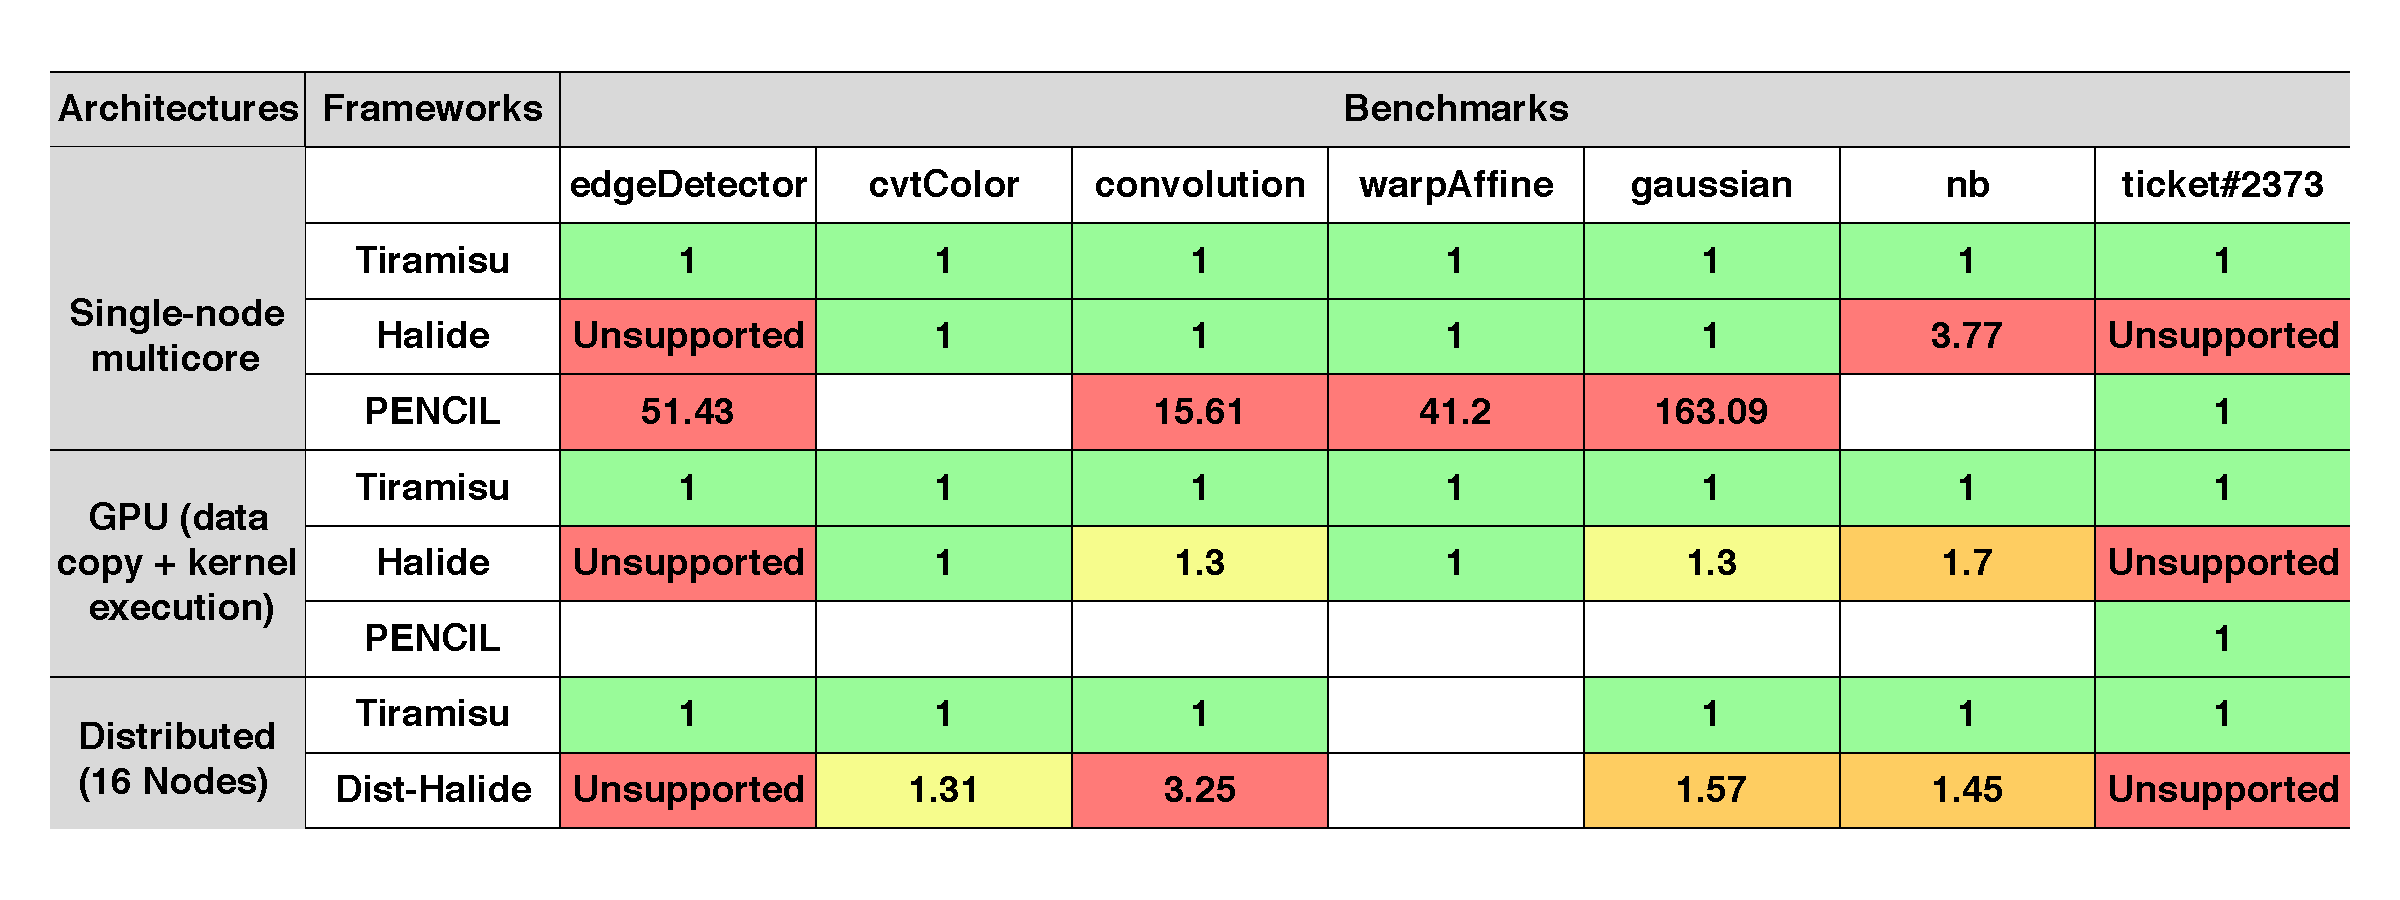
\includegraphics[width=1.05\columnwidth,trim=50 10 10 10]{./figures/tiramisu_heatmap.pdf}
\vspace{-0.5cm}
\caption{A heatmap comparing the normalized execution times of code generated by \framework{} with other frameworks (lower is better).  Comparison is performed on three architectures: single-node multicore, GPU, distributed (16 nodes).}
\label{fig:speedup}

\end{figure}

Figure~\ref{fig:speedup} compares the normalized execution time of code generated by \framework{} to other state-of-the-art frameworks on three architectures: single-node multicore, GPU and distributed (16 nodes).  For the single-node multicore and GPU we compare \framework{} to Halide, an industrial framework that uses a scheduling language, and to PENCIL, a fully automatic polyhedral compiler.  For the distributed architecture, we compare only to Halide since PENCIL does not generate distributed code and the only other polyhedral compiler that generates distributed code (pluto-mpi) does not support non-affine code (4/7 of our benchmarks have non affine code).

\paragraph{Single-node multicore}
In four of the benchmarks, the performance of the code generated by \framework{} matches the performance of Halide.  We use the same schedule for both implementations; these schedules were hand-written by Halide experts.  The results for \texttt{edgeDetector}, \texttt{convolution}, \texttt{warpAffine} and \texttt{gaussian} which have non-affine array accesses and conditionals show that \framework{} handles such pattern efficiently.

Two of the other benchmarks, \texttt{edgeDetector} and \texttt{ticket \#2373}, cannot be implemented in Halide.  The following code snippet shows \texttt{edgeDetector}.
%is an example of a recurrent filter extracted from~\cite{recfilter}, a compiler designed to support recurrent filters.

\vspace{-0.15cm}
\begin{lstlisting}[language=C,escapechar=@,numbers=none]
/* Ring Blur Filter */
R(i,j) = (Img(i-1,j-1) + Img(i-1,j) + Img(i-1,j+1)+
          Img(i,j-1)   +              Img(i,j+1)  +
          Img(i+1,j-1) + Img(i+1,j) + Img(i+1,j+1))/8;
/* Roberts Edge Detection Filter */
Img(i,j) = abs(R(i,j)-R(i+1,j-1)) + abs(R(i+1,j)-R(i,j-1));
\end{lstlisting}
\vspace{-0.15cm}

\texttt{edgeDetector} cannot be implemented in Halide because it creates a cyclic dependence graph with a cycle length $\geq 1$.
Halide can only express programs with an acyclic dependence graph, with some exceptions;  this restriction is imposed by the Halide language and compiler to avoid the need to prove the legality of some optimizations (since proving the legality of certain optimizations is difficult in the Halide interval-based representation).
%in an interval-based representation in the case of a cyclic dependence graph.
\framework{} does not have this restriction since it checks transformation legality using dependence analysis~\cite{feautrier_dataflow_1991}.
%An other example of an a filter that exhibit this pattern include the PatchMatch algorithm~\cite{Barnes:2009:PRC:1531326.1531330}.
%By relying on dependence analysis to check the correctness of optimizations, \framework{} enables Halide to
%and on checking the legality of transformations using the polyhedral model~\cite{konrad_elimination_2011} to decide whether a transformation can be performed.

In \texttt{ticket \#2373}, which exhibits a triangular iteration domain,  Halide's bounds inference over-approximates the computed bounds which leads the generated code to fail in execution.  This over-approximation in Halide is due to the use of intervals to represent iteration domains, which prevents Halide from performing precise bounds inference for non-rectangular iteration spaces.  \framework{} can handle this case naturally since it relies on a polyhedral based model where sets can include any affine constraint  in addition to loop bounds.  These examples show that the model exposed by \framework{} naturally supports more complicated code patterns than an advanced, mature DSL compiler.

For \texttt{nb}, the code generated from \framework{} achieves $3.77\times$ speedup over the Halide-generated code. This is primarily due to loop fusion.  In this code, \framework{} enhances data locality by fusing loops into one loop;  this is not possible in Halide, which cannot fuse loops if they update the same buffer.  Halide makes this conservative assumption because otherwise it cannot prove the fusion is correct. This is not the case for \framework{} which uses dependence analysis to prove correctness.

In comparison with PENCIL, the main difference is that both \framework{} and Halide apply vectorization and unrolling on the innermost loops while PENCIL does not.  Most of the benchmarks have many statements within the innermost loop, therefore vetorizing the innermost loop transforms all of those statements to their vector equivalent while unrolling increases register reuse and instruction level parallelism.

\paragraph{GPU}
For the GPU backend, the reported times are the total execution times (data copy and kernel execution).
Code generated by \framework{} for \texttt{convolution} and \texttt{gaussian} is faster than that of Halide because code generated by \framework{} uses constant memory to store the weights array, while the current version of Halide does not use constant memory for its PTX backend.  The only different between the schedule of \framework{} and Halide in these benchmarks is the use of \texttt{tag\_gpu\_constant()} in \framework{}.  Data copy times, for all the filters,  are the same for \framework{} and Halide.

In comparison with PENCIL ...

\begin{figure}[t]
\centering
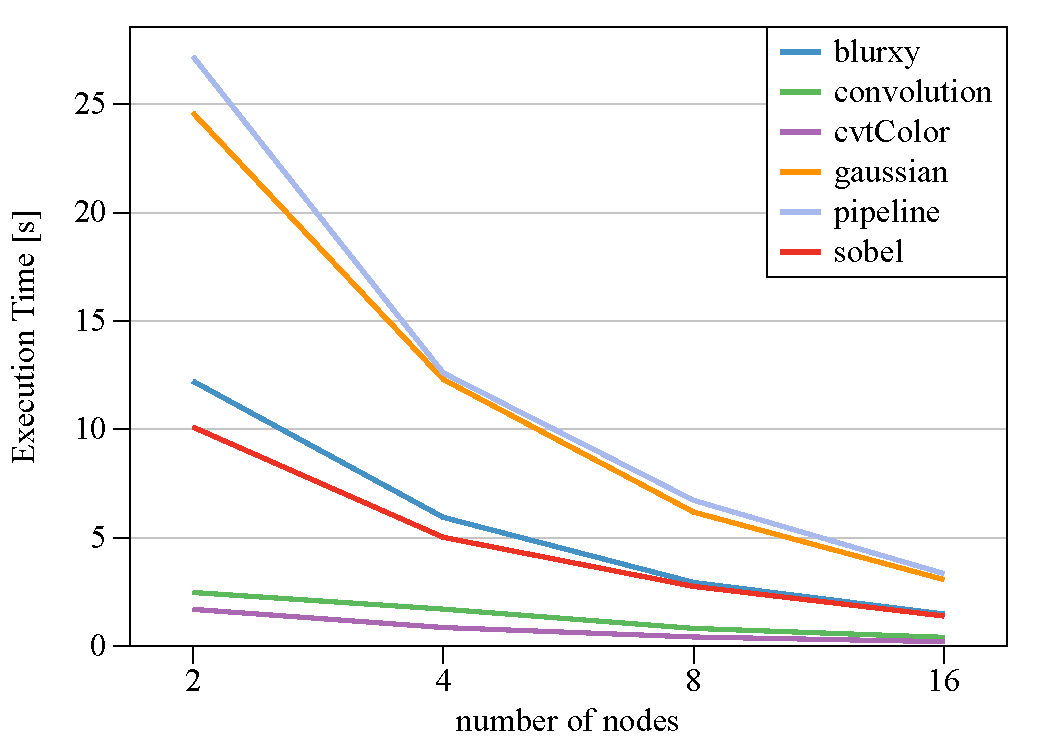
\includegraphics[width=0.6\columnwidth, trim=0 30 0 60]{./figures/tiramisudist}
\caption{Execution time of distributed \framework{} for 2, 4, 8, and 16 nodes}
\label{fig:distCPU_tiramisu_scaling_exec}
%\vspace{-0.5cm}
\end{figure}

\paragraph{Distributed}
We assume the data are already distributed across the nodes by rows. Of these benchmarks, \texttt{nb}, \texttt{cvtColor} and \texttt{ticket \#2373} do not require any communication; the other four require communication due to overlapping boundary regions in the distributed data.

Figure \ref{fig:speedup} compares the execution time of distributed \framework{} and distributed Halide. \framework{} is faster than distributed Halide in each case. For the kernels involving communication, code generated by distributed Halide has two problems compared to \framework{}:  it overestimates the amount of data it needs to send, and it unnecessarily packs together contiguous data into a separate buffer before sending.  Halide distributed always packs the data that need to be sent into a buffer then sends the data (this strategy is useful for the general case but is not needed in this case).

The only difference between the \framework{} and distributed Halide code for these benchmarks is the use of the \texttt{send} and \texttt{receive} scheduling commands in \framework{}.  These commands allow the user to specify exactly the amount of data that need to be sent and also allow the compiler to avoid the unnecessary packing.
%In addition to this, in \framework{}, the user specifies exactly which data should be transferred between nodes so there is no additional run-time overhead.  For the kernels not requiring communication, Halide still has to fully check that the data to send is an empty set (the interval model used in Halide does not allow compile-time emptiness check).

Figure \ref{fig:distCPU_tiramisu_scaling_exec} shows the execution time of the kernels with distributed \framework{} when running on 2, 4, 8, and 16 nodes.  This graph shows that distributed code generated from \framework{} scales well as the number of nodes increases (strong scaling).

\vspace{-0.25cm}
\subsection{Evaluation Summary}

Overall, the experiments demonstrated the use of \framework as an optimization framework for implementing a set of image processing and stencils, for multiple backends.  We show that \framework{} is expressive: it allows Halide to implement new optimizations and algorithms.  The experiments also show that \framework{} is suitable for targeting multiple hardware architectures, such as multicore CPUs, GPUs and distributed systems. Thanks to its flexible scheduling commands, it generates highly optimized code for a variety of of architectures and algorithms.


%\vspace{-0.25cm}
\section{Acknowledgement}
This work was supported by the Applications Driving Architectures (ADA) Research Center, a JUMP Center co-sponsored by SRC and DARPA.

\vspace{-0.25cm}
\section{Conclusion}

In this paper we introduce \framework, an optimization framework that features a scheduling language with scheduling commands for targeting multicore CPUs, GPUs, and distributed systems.  A four-layer intermediate representation that separates the algorithm, the schedule, the data layout and the communication is used to implement the proposed scheduling language.
We evaluate \framework by targeting a variety of backends and demonstrate that it generates code matching and outperforming state-of-the-art frameworks.

\newpage

%\section{Notation and Definitions}

\subsection{Presburger formula\label{presburger}}

We use an EBNF (Extended Backus-Naur Form) grammar to define Presburger formulas.
\[
\begin{array}{lcl}
\pgrammar{formula} & \gets &  \pgrammar{formula} \wedge \pgrammar{formula} \\ 
        & & ~|~ \pgrammar{formula} \vee   \pgrammar{formula} \\
        & & ~|~ \neg \pgrammar{formula} 
        ~|~ \exists \pgrammar{var}. \pgrammar{formula} \\
        & & ~|~ \forall \pgrammar{var}. \pgrammar{formula}
        ~|~ \pgrammar{atom} \\
                            
\pgrammar{atom} & \gets &  \pgrammar{term} \pgrammar{relop} \pgrammar{term}
                            \\
\pgrammar{term} & \gets &     \pgrammar{numeral}
        ~|~ \pgrammar{term} + \pgrammar{term} \\
        & & ~|~ -\pgrammar{term} \\
        & & ~|~ \pgrammar{numeral} * \pgrammar{term}
        ~|~ \pgrammar{var}
                            \\
\pgrammar{relop} & \gets &    <
        ~|~ \leq
                            ~|~ =
                            ~|~ >
                            ~|~ \geq
                            \\
\pgrammar{var} & \gets &      x
                            ~|~ y
                            ~|~ z
                            ~|~ \dots
                            \\
\pgrammar{numeral} & \gets &  0
                            ~|~ 1
                            ~|~ 2
                            ~|~ \dots
                            \\
\end{array}
\]

Note that $\pgrammar{numeral} * \pgrammar{term}$ is not a general multiplication operator;
it is a shortcut for $\pgrammar{term}+\dots+\pgrammar{term}$.

Presburger arithmetic is used mainly because it is a decidable arithmetic.
That is, there exists an algorithm which decides whether an arbitrary Presburger formula is true (valid) or not, which is important for many polyhedral operations.


\subsection{Quasi-Affine Constraints}
\label{qaffine}

A \emph{quasi-affine constraint} is a constraint over integer values and integer variables involving only the operators \lstinline{+}, \lstinline{-}, $\times$, \lstinline{/}, \lstinline{mod}, \lstinline{&&}, \lstinline{||}, \lstinline{<}, \lstinline{<=}, \lstinline{>}, \lstinline{>=}, \lstinline{==}, \lstinline{!=}, and the ternary \lstinline{?:} operator, where the second argument of \lstinline{/} and \lstinline{mod} must be a (positive) integer literal, and where at
least one of the arguments of $\times$
must be a constant expression.
An example of a quasi-affine constraint for a statement in a loop nest is $10\times i+j+n>0$, where $i$ and $j$ are loop iterators and $n$ is a
\emph{symbolic constant} (i.e., a variable that has an unknown but fixed value for the duration of
an execution).  An example of a non-quasi-affine constraint is $i \times i>0$, because we require one of the arguments be a constant.


\section{Integer Sets}

An \emph{integer set} is a set of integer tuples from $\mathbb{Z}^d$ that can be specified using  affine constraints. $d$ is the dimensionality of the set (the number of integers in each tuple) and a d-tuple is represented as $(a_1, a_2, \dots, a_d)$.  An example of a set of integer tuples is:
$$\{(1,1); (2,1); (3,1); (1,2); (2,2); (3,2)\}$$

Instead of listing all the integer tuples of the set, we describe the set using affine constraints:
$$\{S(i,j): 1 \leq i \leq 3 \wedge 1 \leq j \leq 2\}$$

\noindent where $i$ and $j$ are the dimensions of the set.
The tuples of a set can optionally have a common name, such as
$S$ in this example.
Figure~\ref{fig:set} shows a graphical representation of the map $S$.

\begin{figure}[th]
  \begin{minipage}{.22\textwidth}
    \centering
    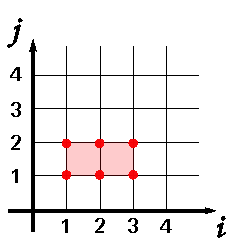
\includegraphics[scale=0.6]{figures/set.pdf}
    \captionof{figure}{Graphical representation of a set}
    \label{fig:set}
  \end{minipage}
  \begin{minipage}{.22\textwidth}
    \centering
    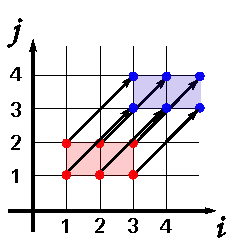
\includegraphics[scale=0.6]{figures/map.pdf}
    \captionof{figure}{Graphical representation of a map}
    \label{fig:map}
  \end{minipage}
\end{figure}

In general, an integer set has the form
$$S = \{N(\vec{s}) | f(\vec{s}, \vec{p})\}$$

\noindent with $\vec{s}$ representing the integer tuples of
the integer set ($\vec{s} \in \mathbb{Z}^d$), $N$, a common name
for all the tuples $\vec{s}$ usually used as the name of computations, $d$ the dimensionality of the set, $\vec{p} \in \mathbb{Z}^e$ a vector of $e$ parameters and $f(\vec{s}, \vec{p})$ a Presburger formula that evaluates to true, if and only if $\vec{s}$ is an element of $S$ for the given parameters $\vec{p}$.

\subsection{Relations (maps)}
A map is a relation between two integer sets.  For example
$$M = \{S1(i,j) \rightarrow S1(i+2,j+2) : 1 \leq i \leq 3 \wedge 1 \leq j \leq 2\}$$

\noindent represents a relation between two sets. The first set
is called the \emph{domain} or the \emph{source}
and the second is called the \emph{range} or the
\emph{sink}.
Figure~\ref{fig:map} shows a graphical representation of
the map $M$.


In general, a map has the form
$$M = \{A(\vec{s}) \rightarrow B(\vec{o}), (\vec{s}, \vec{o}) \in \mathbb{Z}^{d_1}\times\mathbb{Z}^{d_2} | f(\vec{s}, \vec{o}, \vec{p})\}$$

\noindent where $A(\vec{s})$ represents the domain or the
source and $B(\vec{o})$ represents the range or the sink.
$d_1$ and $d_2$ are the dimensionalities of $\vec{s}$
and $\vec{o}$, $\vec{p} \in \mathbb{Z}^e$ is a vector of $e$ parameters and $f(\vec{s}, \vec{o}, \vec{p})$ is a Presburger formula that evaluates to true if and only if there is a relation from $\vec{s}$ to $\vec{o}$ in $M$ for the given parameters
$\vec{p}$.

\section{Three-Layer IR}
\label{appendixlayers}
\subsection{Layer I: \Layerone}

The first layer is a union of \emph{computation sets} such that each computation set describes one statement in the program. Each computation set is defined as follows:
$$\{N1(\vec{s}) | f(\vec{s}, \vec{p})\} : g(N2(\vec{s}), N3(\vec{s}), ..., N4(\vec{s}))$$

\noindent where $N1(\vec{s})$ is a computation that has the name $N1$, and where $g(N2(\vec{s}), N3(\vec{s}), ..., N4(\vec{s}))$ is the expression that the computation computes and $f(\vec{s}, \vec{p})$ is a Presburger formula that evaluates to true, if and only if $\vec{s}$ is an element of $S$ for the given parameters $\vec{p}$.


\subsection{Layer II: \Layertwo}

The second layer is identical to the first layer except that computations in this layer are ordered based on their lexicographical order.

\subsection{Layer III: \Layerthree}
\label{layer3}

The third layer is a union of computation sets and a set of access relations.  The computation sets are identical to the Layer II computation sets except that new allocation/deallocation statements are added.  The set of access relations is described as follows:
$$\{N1(\vec{s}) \rightarrow B(\vec{o}), (\vec{s}, \vec{o}) \in \mathbb{Z}^{d_1}\times\mathbb{Z}^{d_2} | f(\vec{s}, \vec{o}, \vec{p})\}$$

\noindent where $N1(\vec{s})$ is a computation mapped to the buffer element $B[\vec{o}]$ and $f(\vec{s}, \vec{o}, \vec{p})$ is a Presburger formula that evaluates to true if and only if there is a relation from $\vec{s}$ to $\vec{o}$ for the given parameters $\vec{p}$.

\begin{figure}
\small

\centering\begin{lstlisting}[language=C,escapechar=@,basicstyle=\linespread{0.9}\small\ttfamily]
for (i in 0..N)
  for (j in 0..M)
    S1
    S2
\end{lstlisting}
(a) Original computation expressed as an imperative program


\begin{tabular}{c|c}
\\\hline
   \begin{tabular}{l@{\hspace{4pt}}r@{\hspace{2pt}}c@{\hspace{2pt}}c@{\hspace{2pt}}c@{\hspace{0pt}}l}
    S1: & ( & $i,$ & $j$, & $0$ & ) \\
    S2: & ( & $i$, & $j$, & 1 & ) \\
    \multicolumn{6}{c}{ (b) Sequential}
   \end{tabular}
     &  
   \begin{tabular}{l@{\hspace{4pt}}r@{\hspace{2pt}}c@{\hspace{2pt}}c@{\hspace{2pt}}c@{\hspace{0pt}}l}
    S1: & ( & $j$, & $i$, & 0 & ) \\
    S2: & ( & $j$, & $i$, & 1 & ) \\
    \multicolumn{6}{c}{ (c) Transposed}
   \end{tabular} \\\hline

    \begin{tabular}{l@{\hspace{4pt}}r@{\hspace{2pt}}c@{\hspace{2pt}}c@{\hspace{2pt}}c@{\hspace{0pt}}l}
    S1: & ( & $i$, & 0, & $j$ & ) \\
    S2: & ( & $i$, & 1, & $j$ & ) \\
    \multicolumn{6}{c}{ (d) Inner loop fission}
   \end{tabular} 
   & 
    \begin{tabular}{l@{\hspace{4pt}}r@{\hspace{2pt}}c@{\hspace{2pt}}c@{\hspace{2pt}}c@{\hspace{0pt}}l}
    S1: & ( & 0, & $i$, & $j$ & ) \\
    S2: & ( & 1, & $i$, & $j$ & ) \\
    \multicolumn{6}{c}{ (e) Outer loop fission}
   \end{tabular} \\\hline
   
    \begin{tabular}{l@{\hspace{4pt}}r@{\hspace{2pt}}c@{\hspace{2pt}}c@{\hspace{2pt}}c@{\hspace{2pt}}c@{\hspace{0pt}}l}
    S1: & (  & $i/N$, & $i\%N$, & $j$, & 0 & ) \\
    S2: & (  & $i/N$, & $i\%N$, & $j$, & 1 & ) \\
    \multicolumn{6}{c}{ (f) Loop split}
   \end{tabular} 
   &
    \begin{tabular}{l@{\hspace{4pt}}r@{\hspace{2pt}}c@{\hspace{2pt}}c@{\hspace{2pt}}c@{\hspace{2pt}}c@{\hspace{0pt}}l}
    S1: & ( & $i/N$, & $j$, & $i\%N$, & 0 & ) \\
    S2: & ( & $i/N$, & $j$, & $i\%N$, & 1 & ) \\
    \multicolumn{6}{c}{ (g) ... \& permuted}
    \end{tabular}  \\\hline
    
    \begin{tabular}{l@{\hspace{4pt}}r@{\hspace{2pt}}c@{\hspace{2pt}}c@{\hspace{2pt}}c@{\hspace{2pt}}c@{\hspace{0pt}}l}
    S1: & ( & $i\%P$ {\it (cpu)}, & $j$, & $i/P$, & 0 & ) \\
    S2: & ( & $i\%P$ {\it (cpu)}, & $j$, & $i/P$, & 1 & ) \\
    \multicolumn{6}{c}{ (h) Outer parallel }
   \end{tabular} 
   &
    \begin{tabular}{l@{\hspace{4pt}}r@{\hspace{2pt}}c@{\hspace{2pt}}c@{\hspace{2pt}}c@{\hspace{2pt}}c@{\hspace{0pt}}l}
    S1: & ( & $i$, & $j/4$, & 0, & $j\%4$ {\it (vec)} & ) \\
    S2: & ( & $i$, & $j/4$, & 1, & $j\%4$ {\it (vec)} & ) \\
    \multicolumn{6}{c}{ (i) Inner vectorized }
   \end{tabular} \\ 

\end{tabular}
 \caption{For a simple loop next with two statements, examples of different time-processor vectors leading to many possible execution arrangements. }
\label{fig:time-processor-vector}
\end{figure}

\subsection{Time-Processor Vectors}

% to map an iteration into a \processor and time order.
The {\it time-\processor vector} in Layer II is a vector indicates the logical time of execution of computations and the processor on which they should be executed.
%Computations in Layer II are represented as {\it time-\processor vectors}.
Each one of those vectors has a name associated to it (the name of the computation). $S1(0,0,0)$, $S2(0,0,1)$, $S1(i,j,0)$ and $S2(i(cpu),j,1)$ are  examples of time-\processor vectors representing computations in Layer II.
In general, the  time-\processor vector has two types of dimensions: time dimensions and \processor dimensions.
The time dimensions provide the logical order of execution of the computations while the \processor dimensions indicate on which processor the computations should be executed.
In the previous example, the first three vectors have time dimensions only, while the last vector has one space dimension.
We use a tag to indicate that a given dimension is a \processor dimension; this tag indicates mainly the type of processor to which the computations are mapped.%: cpu, gpu, node (for a distributed system), etc.

Assuming that we have two time-\processor vectors we want to know which vector among the two executes first, then all we need to do is to compare the two vectors lexicographically~\footnote{A \emph{time-\processor vector} $(i_1, \dots, i_k, \dots, i_n)$ lexicographically precedes another time-\processor vector $(i_1', \dots, i_k', \dots, i_n')$ if and only if $\exists k \in \mathbb{N}$ such that $i_1 = i_1' \wedge i_2 = i_2' \wedge \dots \wedge i_k < i_k'$}.
In the example, $S1(0,0,0]$ precedes $S2(0,0,1)$ lexicographically, so $S1(0,0,0)$ is scheduled to be executed before $S2(0,0,1)$.
The ability to add dimensions and reorder them freely enables the expression of multiple possible mappings from the original iteration space of the computations to complex execution scenarios.
Figure~\ref{fig:time-processor-vector} provides examples of different optimizations for a simple algorithm and shows the  time-\processor vectors used to express those optimizations.
Each of the dimensions of the vector can be an indexed variable, distributing the computation over that dimension or a constant providing a lexical ordering between statements. 
The algorithms will be using a custom intermediate representation within each DSL, however, we use a classical imperative language representation to describe them in this paper.
A value can be annotated by a processor type, indicating where that computation will be placed, and indicating that dimension will be run in parallel.

\bibliography{bibliography}

\end{document}
